
% !TEX program = pdflatex
\documentclass[aspectratio=169,10pt]{beamer}

% ----------------------
% Theme / look
% ----------------------
\usetheme{Madrid}
\usecolortheme{default}
\setbeamertemplate{navigation symbols}{}
\setbeamertemplate{caption}[numbered]
\usefonttheme{professionalfonts}

% --- Remove footline entirely (fixes Notability/iPad annotation blocking) ---
\setbeamertemplate{footline}{}

% --- Disable PDF hyperlink boxes (fixes Notability annotation blocking) ---
\hypersetup{draft=true}

% ----------------------
% Packages
% ----------------------
\usepackage{amsmath, amssymb, bm}
\usepackage{graphicx}
\usepackage{booktabs, tabularx}
\usepackage{mathtools}
\usepackage{siunitx}
\usepackage{tikz}
\usepackage{pgfplots}
\pgfplotsset{compat=1.18}
\usetikzlibrary{arrows.meta, positioning, calc, shapes, decorations.pathreplacing}

\usepackage[most]{tcolorbox}
\usepackage{listings}
\usepackage{xcolor}

% ----------------------
% Graphics
% ----------------------
\graphicspath{{Figures/}}

% ----------------------
% Listings (MATLAB)
% ----------------------
\lstdefinelanguage{Matlab}{
  keywords={break,case,catch,continue,else,elseif,end,for,function,global,if,otherwise,persistent,return,switch,try,while},
  morekeywords={sdpvar,optimize,sdpsettings,quadprog,linprog,value,optimoptions,disp,fprintf,clear,clc,max,exp,sin,ones},
  sensitive=true,
  morecomment=[l]\%,
  morestring=[m]'
}
\lstset{
  language=Matlab,
  basicstyle=\ttfamily\scriptsize,
  keywordstyle=\color{blue!70!black}\bfseries,
  commentstyle=\color{green!40!black},
  stringstyle=\color{orange!70!black},
  numbers=left,
  numberstyle=\tiny\color{gray!70},
  stepnumber=1,
  numbersep=6pt,
  tabsize=2,
  showstringspaces=false,
  breaklines=true,
  breakatwhitespace=false,
  frame=single,
  rulecolor=\color{gray!40}
}

% ----------------------
% Box styles (match your notes vibe)
% ----------------------
\tcbset{
  beamer,
  enhanced,
  colback=white,
  colframe=blue!60!black,
  boxrule=0.6pt,
  arc=2pt,
  left=6pt,right=6pt,top=4pt,bottom=4pt
}
\newtcolorbox{defnbox}[1]{title=#1, colframe=blue!70!black, colback=blue!3}
\newtcolorbox{notebox}[1]{title=#1, colframe=teal!70!black, colback=teal!3}
\newtcolorbox{examplebox}[1]{title=#1, colframe=orange!80!black, colback=orange!3}
\newtcolorbox{alertbox}[1]{title=#1, colframe=red!75!black, colback=red!4}

% ----------------------
% Metadata
% ----------------------
\title[Optimisation (MPC Ch.2)]{Optimisation: The Engine of MPC}
\subtitle{MSc Model Predictive Control --- Chapter 2}
\author{\.Ibrahim K\"u\c c\"ukdemiral}
\institute{Glasgow Caledonian University}
\date{\today}

% ----------------------
% Convenience macros
% ----------------------
\newcommand{\R}{\mathbb{R}}
\newcommand{\Z}{\mathbb{Z}}
\newcommand{\argmin}{\operatorname*{arg\,min}}
\newcommand{\argmax}{\operatorname*{arg\,max}}

\begin{document}

% =========================================================
% Title
% =========================================================
\begin{frame}
  \titlepage
\end{frame}

\begin{frame}{A guiding thought}
\begin{quote}
\itshape
``Since the fabric of the universe is most perfect and the work of a most wise Creator,
nothing at all takes place in the universe in which some rule of maximum or minimum does not appear.''
\end{quote}
\hfill --- \textbf{Leonhard Euler}
\end{frame}

\begin{frame}{Learning Objectives}
After studying this chapter, you should be able to:
\begin{enumerate}
  \item Formulate an engineering problem as a mathematical optimisation problem.
  \item Identify the three components: decision variables, objective function, constraints.
  \item Distinguish between convex and non-convex sets and functions.
  \item Classify problems as LP, QP, or MILP and explain why the distinction matters.
  \item Write and solve optimisation problems in MATLAB using YALMIP.
  \item Explain why convexity guarantees that any local minimum is the global minimum.
\end{enumerate}
\end{frame}

\begin{frame}{Outline}
\tableofcontents
\end{frame}

% =========================================================
% Motivation
% =========================================================
\section{Why optimisation is the engine of MPC}

\begin{frame}{From reactive control to optimisation-based control}
\begin{itemize}
  \item A classical PID controller follows a simple, fixed rule: if the error increases, push back harder. It is reactive and rigid.
  \item An MPC controller does not follow a pre-written rule. At every single time step, it faces a choice and determines the best control action within the given constraints.
  \item This process of systematic selection is called \emph{optimisation}.
  \item If the system model is the map that tells the controller where it \textit{can} go, optimisation is the navigator that decides where it \textit{should} go.
\end{itemize}
\begin{defnbox}{Core idea}
Optimisation provides the mathematical framework for translating engineering objectives into computable control actions.
\end{defnbox}
\end{frame}

\begin{frame}{What does optimisation buy us in control?}
\begin{itemize}
  \item A clean way to encode trade-offs: tracking vs.\ effort vs.\ safety.
  \item A uniform way to handle constraints (actuators, states, safety envelopes).
  \item A natural language for multi-step decision making (horizon-based planning).
  \item A bridge between models (\emph{where we can go}) and goals (\emph{where we should go}).
\end{itemize}
\end{frame}

% =========================================================
% What is optimisation?
% =========================================================
\section{What is optimisation?}

\begin{frame}{Definition and standard form}
\begin{defnbox}{Mathematical Definition of Optimisation}
A numerical approach for seeking a \textbf{best} decision or action from a \textbf{set of alternatives}.
\end{defnbox}

\vspace{0.4em}
\textbf{Generic optimisation problem:}
\begin{equation*}
\begin{aligned}
\min_{x}\quad &J(x)\\
\text{s.t.}\quad &x \in S
\end{aligned}
\end{equation*}
\end{frame}

\begin{frame}{The anatomy of an optimisation problem}
Almost every optimisation problem has three ingredients:
\begin{enumerate}
  \item \textbf{Decision variables} ($x$): knobs the solver can turn.
  \item \textbf{Objective function} ($J$): scalar performance score to minimise.
  \item \textbf{Constraints}: rules defining feasibility ($S$).
\end{enumerate}

\begin{notebox}{In MPC}
Decision variables are typically a \emph{sequence} of future inputs over the prediction horizon.
\end{notebox}
\end{frame}

\begin{frame}{Constraints: inequality vs equality}
\begin{equation*}
\begin{aligned}
\min_x \quad & J(x)\\
\text{s.t.}\quad & g_i(x)\le 0,\quad i=1,\dots,m \qquad \text{(inequalities)}\\
& h_j(x)=0,\quad j=1,\dots,q \qquad \text{(equalities)}
\end{aligned}
\end{equation*}

\begin{notebox}{Study note: Constraint Types}
\begin{itemize}
  \item Inequalities describe ranges: ``speed $\le 100$ km/h''.
  \item Equalities describe strict physics: e.g.\ $F=ma$.
  \item In MPC, system dynamics ($x_{k+1}=Ax_k+Bu_k$) are treated as \textbf{equality constraints}.
\end{itemize}
\end{notebox}
\end{frame}

% =========================================================
% Illustrative examples
% =========================================================
\section{Illustrative examples}

\begin{frame}{Modelling: from story to maths}
Turning a physical/data-driven problem into optimisation form is \textbf{modelling}.

\vspace{0.5em}
A useful systematic approach:
\begin{enumerate}
  \item Identify decision variables (what can we choose?)
  \item Formulate the objective (what means ``best''?)
  \item Define constraints (what must be obeyed?)
\end{enumerate}
\end{frame}

\begin{frame}{Example 1: Maximising box volume (setup)}
\begin{examplebox}{Problem Statement}
A $1\text{m}\times 1\text{m}$ square sheet. Cut squares of side $x$ from corners and fold into an open-top box.
Maximise volume.
\end{examplebox}

\begin{center}
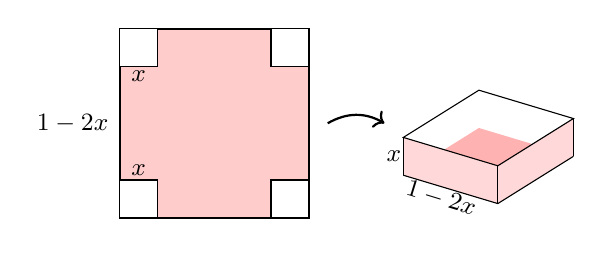
\begin{tikzpicture}[scale=1.2]
  % 2D Sheet
  \fill[red!20] (0,0) rectangle (2,2);
  \draw[thick] (0,0) rectangle (2,2);
  \foreach \xx/\yy in {0/0, 1.6/0, 0/1.6, 1.6/1.6} {
    \fill[white, draw=black] (\xx,\yy) rectangle (\xx+0.4,\yy+0.4);
  }
  \node at (0.2, 1.5) {\small $x$};
  \node at (-0.5, 1) {\small $1-2x$};
  \node at (0.2, 0.5) {\small $x$};

  % Arrow
  \draw[->, thick, bend left] (2.2, 1) to (2.8, 1);

  % 3D Box (simple perspective)
  \begin{scope}[xshift=3cm, yshift=0.45cm]
    \coordinate (A) at (0,0);
    \coordinate (B) at (1.0, -0.3);
    \coordinate (C) at (1.8, 0.2);
    \coordinate (Ah) at (0, 0.4);
    \coordinate (Bh) at (1.0, 0.1);
    \coordinate (Ch) at (1.8, 0.6);
    \coordinate (Dh) at (0.8, 0.9);
    \fill[red!30] (A) -- (B) -- (C) -- (0.8,0.5) -- cycle;
    \fill[red!15] (A) -- (B) -- (Bh) -- (Ah) -- cycle;
    \fill[red!15] (B) -- (C) -- (Ch) -- (Bh) -- cycle;
    \draw (A) -- (B) -- (C);
    \draw (Ah) -- (Bh) -- (Ch) -- (Dh) -- cycle;
    \draw (A) -- (Ah); \draw (B) -- (Bh); \draw (C) -- (Ch);
    \node[rotate=-17] at (0.4, -0.25) {\small $1-2x$};
    \node at (-0.1, 0.2) {\small $x$};
  \end{scope}
\end{tikzpicture}
\end{center}
\end{frame}

\begin{frame}{Example 1: Maximising box volume (model)}
\textbf{Decision variable:} $x$ (corner cut size).

\textbf{Constraints:}
\begin{itemize}
  \item $x\ge 0$ (cut size non-negative)
  \item $2x\le 1 \Rightarrow x\le 0.5$ (cuts cannot overlap)
\end{itemize}

\textbf{Objective (volume):}
\begin{equation*}
V(x)=\underbrace{(1-2x)^2}_{\text{base area}}\cdot \underbrace{x}_{\text{height}} = x(1-2x)^2
\end{equation*}

\begin{notebox}{Standard form trick}
Maximising $f(x)$ is equivalent to minimising $-f(x)$ (so we can use minimisation solvers).
\end{notebox}

\begin{equation*}
\begin{aligned}
\max_x\quad & x(1-2x)^2\\
\text{s.t.}\quad &0\le x\le 0.5
\end{aligned}
\qquad \equiv \qquad
\begin{aligned}
\min_x\quad & -x(1-2x)^2\\
\text{s.t.}\quad &0\le x\le 0.5
\end{aligned}
\end{equation*}
\end{frame}

\begin{frame}{Example 2: Linear regression (least squares)}
\begin{examplebox}{Problem Statement}
Given data $\{(x_i,y_i)\}_{i=1}^N$, fit a line that ``best'' matches the data.
\end{examplebox}

\begin{center}
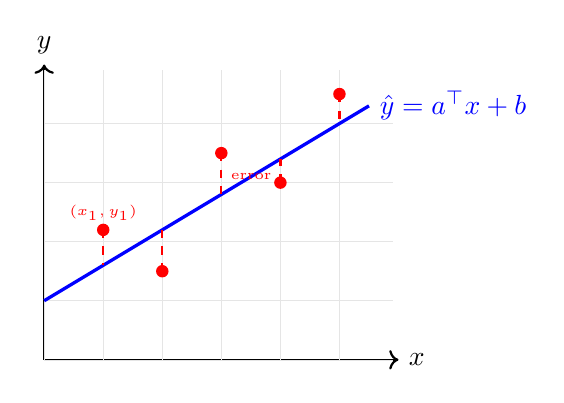
\begin{tikzpicture}[scale=0.75]
  % Axes
  \draw[->, thick] (0,0) -- (6,0) node[right] {$x$};
  \draw[->, thick] (0,0) -- (0,5) node[above] {$y$};
  \draw[step=1cm, gray!20, very thin] (0,0) grid (5.9,4.9);

  % The model line
  \draw[blue, very thick] (0,1) -- (5.5, 4.3) node[right] {$\hat{y}=a^\top x+b$};

  % Data points + residuals
  \foreach \p/\xx/\yy in {1/1/2.2, 2/2/1.5, 3/3/3.5, 4/4/3.0, 5/5/4.5} {
    \draw[dashed, red, thick] (\xx,\yy) -- (\xx, {0.6*\xx + 1});
    \fill[red] (\xx,\yy) circle (3pt);
  }
  \node[red, above] at (1, 2.2) {\tiny $(x_1,y_1)$};
  \node[right, red] at (3, 3.1) {\tiny error};
\end{tikzpicture}
\end{center}
\end{frame}

\begin{frame}{Example 2: Linear regression (model)}
In this problem, the $x_i$ are \textbf{data}, not decision variables.

\textbf{Decision variables:} slope vector $a\in \R^n$ and intercept $b\in \R$.

\textbf{Prediction:} $\hat{y}_i=a^\top x_i + b$.

\textbf{Objective:} minimise the sum of squared errors:
\begin{equation*}
\min_{a,b}\ \sum_{i=1}^N (y_i-\hat{y}_i)^2
=\min_{a,b}\ \sum_{i=1}^N \left(y_i-(a^\top x_i+b)\right)^2
\end{equation*}

\textbf{Constraints:} none (unconstrained).
\end{frame}

% =========================================================
% Multi-variable optimisation ingredients
% =========================================================
\section{Multi-variable optimisation ingredients}

\begin{frame}{The decision vector}
In engineering, we usually choose many values at once.

\begin{equation*}
x=\begin{bmatrix}x_1\\x_2\\\vdots\\x_n\end{bmatrix}\in\R^n
\end{equation*}

\begin{itemize}
  \item The objective maps vector $\rightarrow$ scalar: $J:\R^n\to \R$.
  \item In MPC: if horizon $N=10$ and 2 inputs, decision dimension is $n=20$ (a \emph{sequence} of inputs).
\end{itemize}
\end{frame}

\begin{frame}{Why $J:\R^n\to \R$? The shopping basket analogy (1/2)}
\textbf{Vector of choices:}
\begin{equation*}
x=\begin{bmatrix}2\\6\\1\end{bmatrix}
\quad\leftarrow\ \text{(Bread, Eggs, Milk)}
\end{equation*}

\textbf{The till applies a rule (prices) to produce a single number:}
\begin{equation*}
J(x)=(2\times \pounds 1.00) + (6\times \pounds 0.20) + (1\times \pounds 0.80)
\end{equation*}

\begin{center}
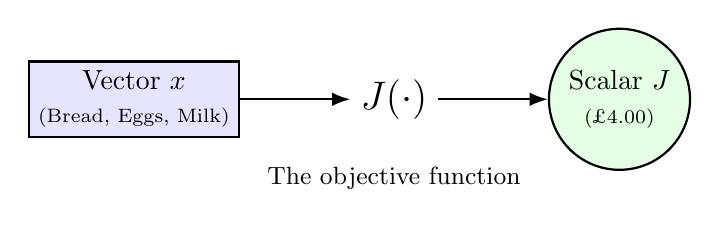
\begin{tikzpicture}[node distance=1.8cm, auto, >=Latex, thick]
  \node [draw, rectangle, align=center, fill=blue!10, minimum height=2.4em] (vector)
  {Vector $x$\\ \scriptsize (Bread, Eggs, Milk)};
  \node [right=1.4cm of vector] (func) {\Large $J(\cdot)$};
  \node [draw, circle, align=center, fill=green!10, right=1.4cm of func, minimum size=2.4em] (scalar)
  {Scalar $J$\\ \scriptsize (\pounds 4.00)};
  \draw [->] (vector) -- (func);
  \draw [->] (func) -- (scalar);
  \node [below=0.35cm of func] {\small The objective function};
\end{tikzpicture}
\end{center}
\end{frame}

\begin{frame}{Why $J:\R^n\to \R$? The shopping basket analogy (2/2)}
\begin{itemize}
  \item You can't easily compare two baskets by looking at item-by-item counts.
  \item After mapping to a scalar (total price), comparison is immediate.
\end{itemize}

\begin{notebox}{Key takeaway}
Optimisation algorithms cannot minimise a list/vector. They minimise a \textbf{single number}.
The objective function is the translator from complex engineering decisions to a scalar score.
\end{notebox}

\begin{itemize}
  \item In MPC, Plan A may track better but use more fuel than Plan B.
  \item $J(x)$ compresses all trade-offs so we can rank plans.
\end{itemize}
\end{frame}

\begin{frame}{Constraints and the feasible set}
Constraints define a region of allowable decisions.

\begin{itemize}
  \item Inequalities: $g_i(x)\le b_i$ (bounds, safety).
  \item Equalities: $h_j(x)=0$ (physics, model dynamics).
  \item Domain restrictions: $x\in\R^{n-p}\times\Z^p$ (discrete logic) --- usually hard.
\end{itemize}

\begin{equation*}
S=\{x\in\R^n \mid g_i(x)\le b_i\ \forall i,\ \ h_j(x)=0\ \forall j\}
\end{equation*}

\begin{alertbox}{Infeasibility}
If constraints conflict and the intersection is empty, the problem has \textbf{no solution}.
\end{alertbox}
\end{frame}

\begin{frame}{Infeasibility and empty feasible sets}
\begin{alertbox}{What if constraints contradict each other?}
If the intersection of all constraints is the \textbf{empty set}, the problem is \textbf{infeasible} --- no solution exists.
\end{alertbox}

\textbf{Example:} $x \le 2$ and $x \ge 5$ simultaneously --- no $x$ satisfies both.

\vspace{0.5em}
\textbf{In MPC:} Infeasibility can arise when:
\begin{itemize}
  \item The prediction horizon is too short to satisfy terminal constraints.
  \item State constraints are too tight relative to the disturbance level.
  \item The system starts too far from the target.
\end{itemize}

\begin{notebox}{Practical remedy}
Use \textbf{soft constraints} (add a penalty for violation instead of a hard limit) to ensure the MPC always has a feasible solution.
\end{notebox}
\end{frame}

\begin{frame}{Visualising a feasible set (intersection of constraints)}
\begin{examplebox}{Example}
In $\R^2$, constrain points to be:
\begin{enumerate}
  \item Inside a circle: $x_1^2+x_2^2\le 4$
  \item Above a cubic: $x_2\ge x_1^3$
\end{enumerate}
Feasible set $S$ is their intersection.
\end{examplebox}

\begin{center}
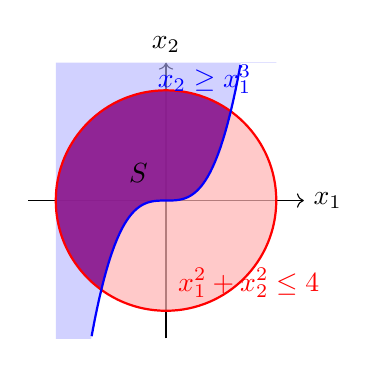
\begin{tikzpicture}[scale=.7]
  \draw[->] (-2.5,0) -- (2.5,0) node[right] {$x_1$};
  \draw[->] (0,-2.5) -- (0,2.5) node[above] {$x_2$};

  \fill[red!30, opacity=0.7] (0,0) circle (2cm);

  \begin{scope}
    \clip (-2.5, -2.5) rectangle (2.5, 2.5);
    \fill[blue!30, opacity=0.6] plot[domain=-2:2, samples=60] (\x, {\x*\x*\x}) |- (-2,2.5) -- cycle;
  \end{scope}

  \begin{scope}
    \clip (0,0) circle (2cm);
    \fill[blue!50!red, opacity=0.8] plot[domain=-1.3:1.3, samples=60] (\x, {\x*\x*\x}) |- (-2,2.5) -- (-2, -2.5) -- cycle;
  \end{scope}

  \draw[thick, red] (0,0) circle (2cm);
  \node[red] at (1.5, -1.5) {$x_1^2+x_2^2\le 4$};

  \draw[thick, blue, domain=-1.35:1.35, samples=60] plot (\x, {\x*\x*\x});
  \node[blue] at (0.7, 2.2) {$x_2\ge x_1^3$};

  \node at (-0.5, 0.5) {\textbf{$S$}};
\end{tikzpicture}
\end{center}
\end{frame}

% =========================================================
% Minimisation vs maximisation, min vs argmin
% =========================================================
\section{Standard form and notation}

\begin{frame}{Min vs.\ argmin (what does the solver return?)}
\begin{itemize}
  \item $\min f(x)$ returns the \textbf{value} of the function at the minimum.
  \item $\argmin f(x)$ returns the \textbf{argument} $x^\star$ that achieves it.
\end{itemize}

\begin{notebox}{In MPC}
We typically care about $\argmin$ because we need the \emph{input} to apply, not just the cost value.
\end{notebox}
\end{frame}

\begin{frame}{Maximisation vs.\ minimisation}
Most numerical solvers are written for \textbf{minimisation}.

\begin{equation*}
\argmax_{x\in S} f(x)\ \equiv\ \argmin_{x\in S} \{-f(x)\}
\end{equation*}

\begin{center}
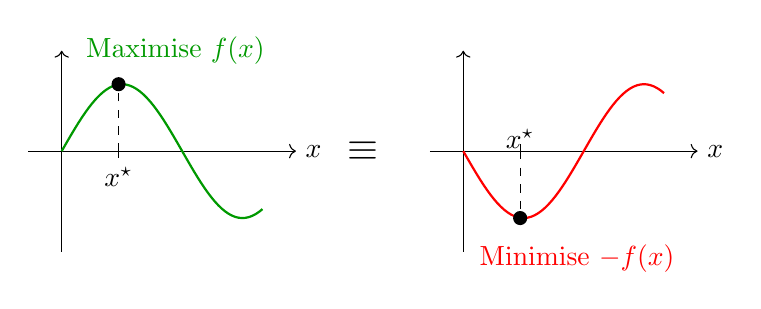
\begin{tikzpicture}[scale=0.85]
  % Maximisation plot
  \begin{scope}
    \draw[->] (-0.5,0) -- (3.5,0) node[right] {$x$};
    \draw[->] (0,-1.5) -- (0,1.5);
    \draw[thick, green!60!black] plot[domain=0:3, samples=60] (\x, {sin(\x*100)});
    \node[green!60!black] at (1.7, 1.5) {Maximise $f(x)$};
    \draw[dashed] (0.85, 0) -- (0.85, 1);
    \draw (0.85, 0.1) -- (0.85, -0.1) node[below] {$x^\star$};
    \fill[black] (0.85, 1) circle (3pt);
  \end{scope}

  \node at (4.5, 0) {\Large $\equiv$};

  % Minimisation plot
  \begin{scope}[xshift=6cm]
    \draw[->] (-0.5,0) -- (3.5,0) node[right] {$x$};
    \draw[->] (0,-1.5) -- (0,1.5);
    \draw[thick, red] plot[domain=0:3, samples=60] (\x, {-sin(\x*100)});
    \node[red] at (1.7, -1.6) {Minimise $-f(x)$};
    \draw[dashed] (0.85, 0) -- (0.85, -1);
    \draw (0.85, 0.1) -- (0.85, -0.1) node[above] {$x^\star$};
    \fill[black] (0.85, -1) circle (3pt);
  \end{scope}
\end{tikzpicture}
\end{center}
\end{frame}

% =========================================================
% Convexity: sets and functions
% =========================================================
\section{Terminology: geometry and convexity}

\begin{frame}{Why geometry matters}
Some optimisation problems are solvable in milliseconds; others can take hours or fail.

\begin{itemize}
  \item The key distinction is often not just \emph{size}, but \textbf{geometry}.
  \item \textbf{Convexity} is the property that makes problems reliable and fast.
  \item In convex problems: local optimum $\Rightarrow$ global optimum.
\end{itemize}
\end{frame}

\begin{frame}{Convex sets}
\begin{defnbox}{Convex Set}
A set $\mathcal{X}$ is \textbf{convex} iff for any $x,y\in\mathcal{X}$, every convex combination lies in $\mathcal{X}$:
\begin{equation*}
\lambda x + (1-\lambda)y\in\mathcal{X},\quad \forall \lambda\in[0,1].
\end{equation*}
\end{defnbox}

\begin{notebox}{Interpretation}
All line segments starting and ending in $\mathcal{X}$ stay within $\mathcal{X}$.
\end{notebox}
\end{frame}

\begin{frame}{Convex vs non-convex sets (visual)}
\begin{center}
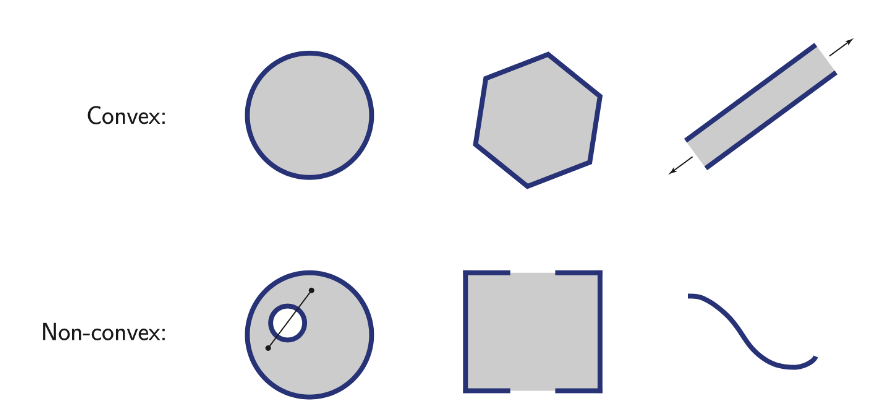
\includegraphics[width=0.75\linewidth,height=0.6\textheight,keepaspectratio]{convex_sets}
\end{center}
\vspace{-0.5em}
\begin{notebox}{Rule of thumb}
If the line segment between two points in the set ever leaves the set, it is \textbf{non-convex}.
\end{notebox}
\end{frame}

\begin{frame}{Hyperplanes and half-spaces}
\begin{defnbox}{Hyperplane}
A hyperplane is $\{x\in\R^n\mid a^\top x=b\}$, with normal vector $a\neq 0$.
\end{defnbox}

\begin{defnbox}{Half-space}
A (closed) half-space is $\{x\in\R^n\mid a^\top x\le b\}$.
\end{defnbox}

\begin{notebox}{Key property}
Hyperplanes and half-spaces are always \textbf{convex}. Intersections of half-spaces form polyhedra.
\end{notebox}
\end{frame}

\begin{frame}{Hyperplane vs half-space (geometry)}
\begin{center}
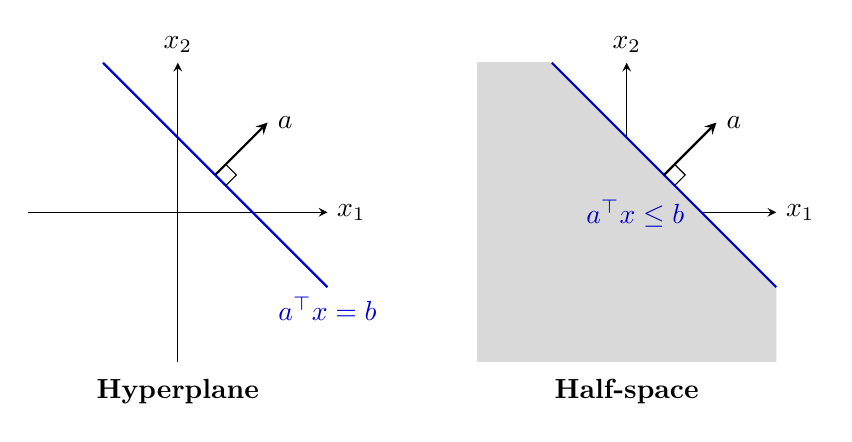
\begin{tikzpicture}[scale=0.95, >=stealth]
  % LEFT: Hyperplane
  \begin{scope}
    \draw[->] (-2,0) -- (2,0) node[right] {$x_1$};
    \draw[->] (0,-2) -- (0,2) node[above] {$x_2$};
    \draw[thick, blue!80!black] (-1, 2) -- (2, -1) node[below] {$a^\top x=b$};
    \draw[->, thick] (0.5, 0.5) -- (1.2, 1.2) node[right] {$a$};
    \draw[rotate around={-45:(0.5,0.5)}] (0.5, 0.7) -- (0.7, 0.7) -- (0.7, 0.5);
    \node at (0, -2.4) {\textbf{Hyperplane}};
  \end{scope}

  % RIGHT: Half-space
  \begin{scope}[xshift=6cm]
    \draw[->] (-2,0) -- (2,0) node[right] {$x_1$};
    \draw[->] (0,-2) -- (0,2) node[above] {$x_2$};
    \begin{scope}
      \clip (-2,-2) rectangle (2,2);
      \fill[gray!30] (-3, 4) -- (4, -3) -- (-3, -3) -- cycle;
    \end{scope}
    \draw[thick, blue!80!black] (-1, 2) -- (2, -1);
    \node[blue!80!black, below left] at (0.9, 0.3) {$a^\top x\le b$};
    \draw[->, thick] (0.5, 0.5) -- (1.2, 1.2) node[right] {$a$};
    \draw[rotate around={-45:(0.5,0.5)}] (0.5, 0.7) -- (0.7, 0.7) -- (0.7, 0.5);
    \node at (0, -2.4) {\textbf{Half-space}};
  \end{scope}
\end{tikzpicture}
\end{center}
\end{frame}

\begin{frame}{Example: linear constraint as a hyperplane}
Consider $2x_1 + x_2 = 2$. This matches $a^\top x=b$ with
\begin{equation*}
a=\begin{pmatrix}2\\1\end{pmatrix},\quad x=\begin{pmatrix}x_1\\x_2\end{pmatrix},\quad b=2.
\end{equation*}

\textbf{Gradient connection:} define $f(x)=2x_1+x_2-2$. Then
\begin{equation*}
\nabla f = \begin{pmatrix}\frac{\partial f}{\partial x_1}\\[4pt]\frac{\partial f}{\partial x_2}\end{pmatrix}
= \begin{pmatrix}2\\1\end{pmatrix}=a,
\end{equation*}
so the gradient is normal to the level set (the line).
\end{frame}

\begin{frame}{Geometry of $2x_1+x_2=2$ and the normal vector}
\begin{center}
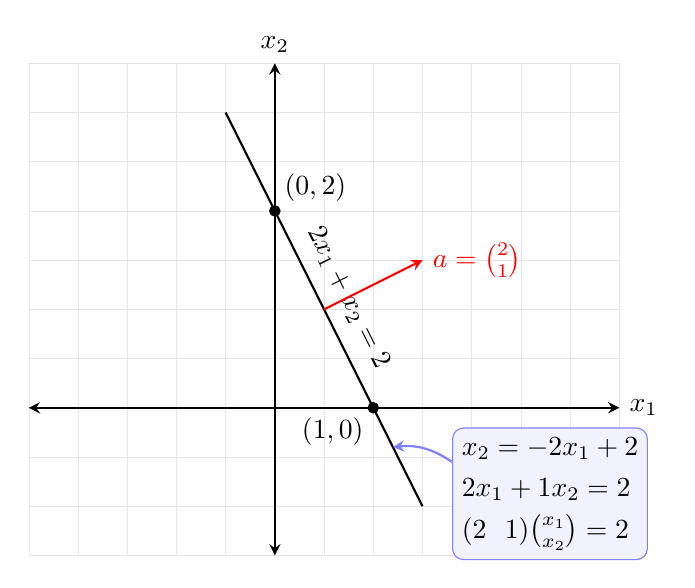
\begin{tikzpicture}[scale=1.25, >=stealth]
  \draw[step=0.5cm, gray!20, very thin] (-2.5,-1.5) grid (3.5,3.5);
  \draw[<->, thick] (-2.5,0) -- (3.5,0) node[right] {$x_1$};
  \draw[<->, thick] (0,-1.5) -- (0,3.5) node[above] {$x_2$};

  \draw[thick, black] (-0.5, 3) -- (1.5, -1) node[midway, sloped, above, yshift=2pt] {$2x_1 + x_2 = 2$};

  \filldraw (0,2) circle (1.5pt) node[above right] {$(0,2)$};
  \filldraw (1,0) circle (1.5pt) node[below left] {$(1,0)$};

  \coordinate (P) at (0.5, 1);
  \draw[->, red, thick] (P) -- ++(1, 0.5) node[right] {$a=\binom{2}{1}$};

  \node[draw=blue!50, fill=blue!5, rounded corners, align=left, anchor=north west]
  at (1.8, -0.2) {
    $x_2=-2x_1+2$ \\[0.3em]
    $2x_1+1x_2=2$ \\[0.3em]
    $(2\ \ 1)\binom{x_1}{x_2}=2$
  };
  \draw[->, blue!50, thick, bend right=20] (1.8, -0.55) to (1.2, -0.4);
\end{tikzpicture}
\end{center}
\end{frame}

\begin{frame}{Polyhedra and polytopes}
\begin{defnbox}{Polyhedron}
A polyhedron is an intersection of finitely many closed half-spaces:
\begin{equation*}
P=\{x\in\R^n\mid a_i^\top x\le b_i,\ i=1,\dots,m\}=\{x\in\R^n\mid Ax\le b\}.
\end{equation*}
\end{defnbox}

\begin{defnbox}{Polytope}
A polytope is a \textbf{bounded} polyhedron.
\end{defnbox}

\begin{alertbox}{Important observation}
Intersections of convex sets are convex. Each half-space is convex $\Rightarrow$ every polyhedron (and polytope) is convex.
Unions of convex sets are \textbf{not} convex in general.
\end{alertbox}
\end{frame}

\begin{frame}{Numerical example: a polytope in $\R^2$}
Constraints:
\begin{align*}
x_1&\ge 0,& x_2&\ge 0,\\
x_1&\le 3,& x_2&\le 2,\\
x_1+x_2&\le 4.
\end{align*}

Standard form $Ax\le b$:
\begin{equation*}
A=\begin{bmatrix}
-1&0\\ 0&-1\\ 1&0\\ 0&1\\ 1&1
\end{bmatrix},\quad
b=\begin{bmatrix}0\\0\\3\\2\\4\end{bmatrix}.
\end{equation*}

Vertices: $(0,0),(3,0),(3,1),(2,2),(0,2)$.
\end{frame}

\begin{frame}{Polytope visualisation}
\begin{center}
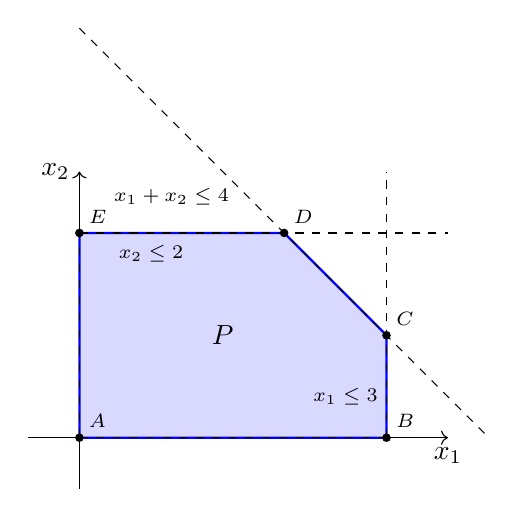
\begin{tikzpicture}[scale=1.3]
  \draw[->] (-0.5,0) -- (3.6,0) node[below] {$x_1$};
  \draw[->] (0,-0.5) -- (0,2.6) node[left] {$x_2$};

  \fill[blue!15] (0,0) -- (3,0) -- (3,1) -- (2,2) -- (0,2) -- cycle;
  \draw[thick,blue] (0,0) -- (3,0) -- (3,1) -- (2,2) -- (0,2) -- cycle;

  \draw[dashed] (0,0) -- (3.6,0);
  \draw[dashed] (0,0) -- (0,2.6);
  \draw[dashed] (3,0) -- (3,2.6);
  \draw[dashed] (0,2) -- (3.6,2);
  \draw[dashed] (0,4) -- (4,0);

  \foreach \xx/\yy/\name in {0/0/A, 3/0/B, 3/1/C, 2/2/D, 0/2/E}
    \fill (\xx,\yy) circle (1.2pt) node[above right] {\scriptsize $\name$};

  \node at (0.7,1.8) {\scriptsize $x_2 \le 2$};
  \node at (2.6,0.4) {\scriptsize $x_1 \le 3$};
  \node at (0.9,2.35) {\scriptsize $x_1 + x_2 \le 4$};
  \node at (1.4,1.0) {$P$};
\end{tikzpicture}
\end{center}
\end{frame}

\begin{frame}{Convex functions}
Let $S$ be convex.
\begin{defnbox}{Convex Function}
$f:S\to\R$ is convex if for all $z_1,z_2\in S$ and $\lambda\in[0,1]$,
\begin{equation*}
f(\lambda z_1+(1-\lambda)z_2)\le \lambda f(z_1)+(1-\lambda)f(z_2).
\end{equation*}
Geometrically: the chord between two points lies above the graph.
\end{defnbox}

\begin{defnbox}{Concave Function}
$f$ is concave if $-f$ is convex (inequality reverses).
\end{defnbox}
\end{frame}

\begin{frame}{Geometric picture of convexity}
\begin{center}
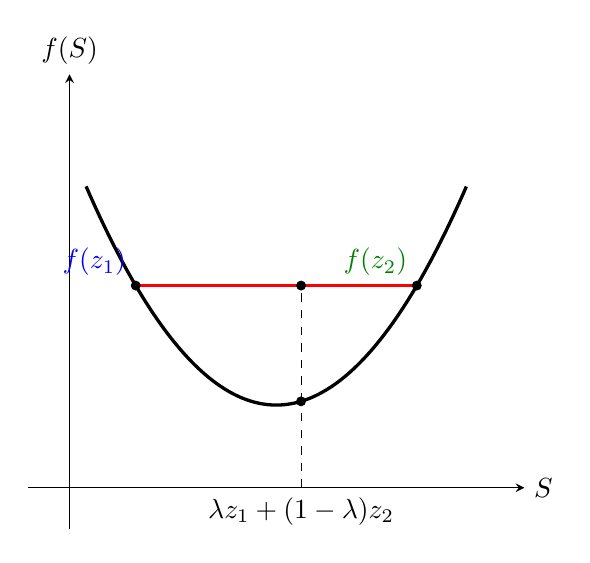
\begin{tikzpicture}[scale=1.05, >=stealth]
  \def\func(\#1){0.5*(\#1-2.5)*(\#1-2.5) + 1}
  \pgfmathsetmacro{\zOne}{0.8}
  \pgfmathsetmacro{\zTwo}{4.2}
  \pgfmathsetmacro{\zMix}{2.8}

  \pgfmathsetmacro{\yOne}{0.5*(\zOne-2.5)*(\zOne-2.5) + 1}
  \pgfmathsetmacro{\yTwo}{0.5*(\zTwo-2.5)*(\zTwo-2.5) + 1}
  \pgfmathsetmacro{\yCurve}{0.5*(\zMix-2.5)*(\zMix-2.5) + 1}
  \pgfmathsetmacro{\slope}{(\yTwo - \yOne) / (\zTwo - \zOne)}
  \pgfmathsetmacro{\yLine}{\yOne + \slope * (\zMix - \zOne)}

  \draw[->] (-0.5,0) -- (5.5,0) node[right] {$S$};
  \draw[->] (0,-0.5) -- (0,5) node[above] {$f(S)$};

  \draw[line width=1.2pt] plot[domain=0.2:4.8, samples=120] (\x, {0.5*(\x-2.5)*(\x-2.5) + 1});
  \draw[red, line width=1.2pt] (\zOne, \yOne) -- (\zTwo, \yTwo);

  \filldraw (\zOne, \yOne) circle (1.5pt) node[above left, text=blue] {$f(z_1)$};
  \filldraw (\zTwo, \yTwo) circle (1.5pt) node[above left, text=green!50!black] {$f(z_2)$};
  \filldraw (\zMix, \yCurve) circle (1.5pt);
  \filldraw (\zMix, \yLine) circle (1.5pt);

  \draw[dashed] (\zMix, 0) -- (\zMix, \yCurve);
  \draw[dashed] (\zMix, \yCurve) -- (\zMix, \yLine);

  \node[below] at (\zMix, 0) {$\lambda z_1+(1-\lambda)z_2$};
\end{tikzpicture}
\end{center}
\end{frame}

\begin{frame}{Why convexity matters for MPC}
\begin{defnbox}{The Fundamental Theorem of Convex Optimisation}
If the objective function $J(x)$ is \textbf{convex} and the feasible set $S$ is \textbf{convex}, then every local minimum is a \textbf{global minimum}.
\end{defnbox}

\vspace{0.5em}
\textbf{Consequence for MPC:}
\begin{itemize}
  \item Linear MPC with quadratic cost and linear constraints $\Rightarrow$ \textbf{convex QP}.
  \item The solver is \emph{guaranteed} to find the best possible control action.
  \item No risk of getting ``stuck'' in a bad local minimum.
  \item Solution can be found \emph{efficiently} (polynomial time).
\end{itemize}

\vspace{0.5em}
\begin{alertbox}{When convexity is lost}
Nonlinear MPC with a nonconvex model may have multiple local minima. The solver may return a suboptimal solution. This is one of the main challenges of nonlinear MPC.
\end{alertbox}
\end{frame}

% =========================================================
% Classification of problems
% =========================================================
\section{Classification of optimisation problems}

\begin{frame}{Two axes of classification}
We commonly classify optimisation problems by:
\begin{enumerate}
  \item \textbf{Constraints:} unconstrained vs constrained (equality/inequality/both).
  \item \textbf{Structure:} linear / quadratic / nonlinear; convex vs nonconvex; continuous vs integer.
\end{enumerate}
\end{frame}

\subsection{Classification I: Existence of constraints}

\begin{frame}{Gradient, Hessian, and optimality}
\textbf{Gradient:} $\nabla J = \begin{bmatrix} \frac{\partial J}{\partial x_1} & \cdots & \frac{\partial J}{\partial x_n} \end{bmatrix}^\top$ --- direction of steepest ascent.

\vspace{0.3em}
\textbf{Hessian:} $\nabla^2 J$ --- matrix of second derivatives. Encodes curvature.

\vspace{0.3em}
\textbf{Necessary condition for a minimum:} $\nabla J(x^\star) = 0$ \quad (stationary point).

\vspace{0.3em}
\textbf{Sufficient condition:} $\nabla J(x^\star) = 0$ \emph{and} $\nabla^2 J(x^\star) \succ 0$ \quad (positive definite Hessian).

\vspace{0.5em}
\begin{notebox}{Connection to convexity}
If $\nabla^2 J(x) \succeq 0$ \emph{everywhere}, then $J$ is convex and any stationary point is a global minimum. For a QP with cost $\frac{1}{2}x^\top P x + q^\top x$, the Hessian is $P$, so convexity $\Leftrightarrow$ $P \succeq 0$.
\end{notebox}
\end{frame}

\begin{frame}{Unconstrained optimisation}
Unconstrained means $x$ can be anywhere in $\R^n$:
\begin{equation*}
\min_{x\in\R^n} J(x)
\end{equation*}

\textbf{Visualisation tool:} level curves (contours) $J(x)=c$.
\begin{notebox}{Topographic map analogy}
Contours represent constant ``height'' (cost). Minimisation finds the smallest attainable contour.
\end{notebox}
\end{frame}

\begin{frame}{Example: level curves of a bowl}
\begin{examplebox}{Unconstrained example}
\[
J(x)=x_1^2+x_2^2
\]
Contours are circles $x_1^2+x_2^2=c$.
\end{examplebox}

\begin{center}
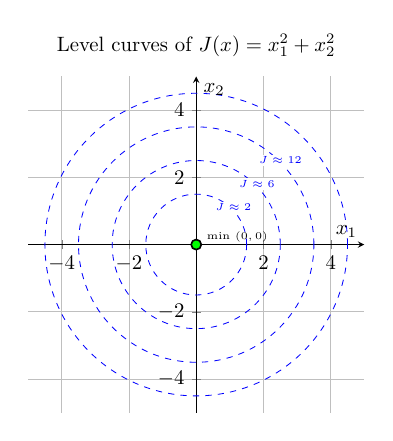
\begin{tikzpicture}[scale=0.75]
\begin{axis}[
  axis lines = middle,
  xlabel = $x_1$,
  ylabel = $x_2$,
  xmin = -5, xmax = 5,
  ymin = -5, ymax = 5,
  axis equal image,
  grid = major,
  xtick = {-4,-2,0,2,4},
  ytick = {-4,-2,0,2,4},
  title = {Level curves of $J(x)=x_1^2+x_2^2$}
]
  \draw[blue, dashed] (axis cs:0,0) circle [radius=1.5];
  \draw[blue, dashed] (axis cs:0,0) circle [radius=2.5];
  \draw[blue, dashed] (axis cs:0,0) circle [radius=3.5];
  \draw[blue, dashed] (axis cs:0,0) circle [radius=4.5];

  \node[blue, font=\tiny, fill=white, inner sep=1pt] at (axis cs: 1.1, 1.1) {$J\approx2$};
  \node[blue, font=\tiny, fill=white, inner sep=1pt] at (axis cs: 1.8, 1.8) {$J\approx6$};
  \node[blue, font=\tiny, fill=white, inner sep=1pt] at (axis cs: 2.5, 2.5) {$J\approx12$};

  \draw[fill=green, draw=black, thick] (axis cs:0,0) circle [radius=0.15];
  \node[anchor=north west] at (axis cs:0.1, 0.6) {\tiny min $(0,0)$};
\end{axis}
\end{tikzpicture}
\end{center}
\end{frame}

\begin{frame}{Constrained optimisation (types)}
We often must enforce limits: $x\in S$.
\begin{itemize}
  \item \textbf{Equality constraints:} $h(x)=0$ restrict to a manifold (curve/surface).
  \item \textbf{Inequality constraints:} $g(x)\le 0$ restrict to a region.
  \item \textbf{General constraints:} both equality and inequality together.
\end{itemize}
\end{frame}

\begin{frame}{Type A: equality constraints (tangent point idea)}
\begin{examplebox}{Problem}
\begin{equation*}
\begin{aligned}
\min_{x}\quad &J(x)=x_1^2+x_2^2\\
\text{s.t.}\quad &h(x)=x_1+2x_2-4=0
\end{aligned}
\end{equation*}
\end{examplebox}

\begin{center}
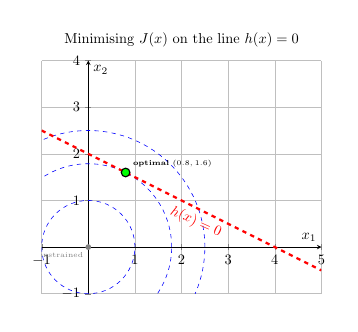
\begin{tikzpicture}[scale=0.52]
\begin{axis}[
  axis lines = middle,
  xlabel = $x_1$,
  ylabel = $x_2$,
  xmin = -1, xmax = 5,
  ymin = -1, ymax = 4,
  axis equal image,
  grid = major,
  title = {Minimising $J(x)$ on the line $h(x)=0$}
]
  \draw[blue, dashed] (axis cs:0,0) circle [radius=1];
  \draw[blue, dashed] (axis cs:0,0) circle [radius=1.788];
  \draw[blue, dashed] (axis cs:0,0) circle [radius=2.5];
  \addplot[domain=-1:5, samples=2, color=red, ultra thick, dashed] {2 - 0.5*x};
  \node[red, rotate=-24, anchor=south] at (axis cs: 2.2, 0.3) {$h(x)=0$};

  \fill[gray] (axis cs:0,0) circle (2pt) node[below left] {\tiny unconstrained};
  \fill[green, draw=black, thick] (axis cs:0.8, 1.6) circle (3pt);
  \node[anchor=south west] at (axis cs:0.85, 1.6) {\tiny \textbf{optimal} $(0.8,1.6)$};
\end{axis}
\end{tikzpicture}
\end{center}

\begin{notebox}{Geometric rule}
The constrained optimum occurs where the constraint is tangent to a level curve.
\end{notebox}
\end{frame}

\begin{frame}[fragile]{Type B: inequality constraints + YALMIP workflow}
\begin{examplebox}{Problem}
\[
\min\; J(x)=x_1^2+x_2^2
\quad \text{s.t.}\quad
\begin{cases}
-x_1-2x_2+5\le 0\\
2x_1+x_2-5\le 0\\
x_1\ge 0,\ x_2\ge 0
\end{cases}
\]
\end{examplebox}

\textbf{YALMIP pattern:} Define variables $\rightarrow$ define objective $\rightarrow$ define constraints $\rightarrow$ solve.
\end{frame}

\begin{frame}[fragile]{Inequality constraints: YALMIP implementation}
\begin{lstlisting}
% 1. Define Decision Variables
x = sdpvar(2,1);

% 2. Define Objective
J = x(1)^2 + x(2)^2;

% 3. Define Constraints (vectorised list)
Constraints = [ -x(1) - 2*x(2) + 5 <= 0, ...
                 2*x(1) +   x(2) - 5 <= 0, ...
                 x(1) >= 0, ...
                 x(2) >= 0 ];

% 4. Solve
optimize(Constraints, J);

% 5. Extract Result
x_star = value(x)   % Expected: (1, 2)
\end{lstlisting}
\end{frame}

\begin{frame}{Inequality constraints: geometric interpretation}
\begin{center}
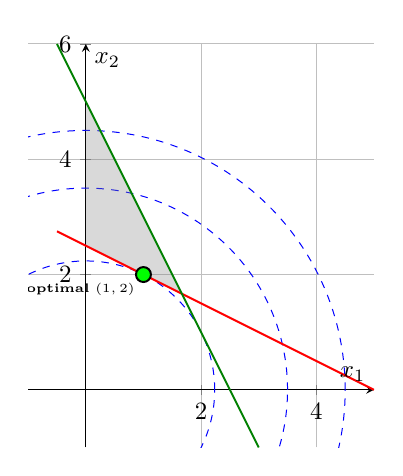
\begin{tikzpicture}[scale=0.9]
\begin{axis}[
  axis lines = middle,
  xlabel = $x_1$,
  ylabel = $x_2$,
  xmin = -1, xmax = 5,
  ymin = -1, ymax = 6,
  axis equal image,
  grid = major
]
  \draw[blue, dashed] (axis cs:0,0) circle [radius=2.236];
  \draw[blue, dashed] (axis cs:0,0) circle [radius=3.5];
  \draw[blue, dashed] (axis cs:0,0) circle [radius=4.5];

  \fill[gray, opacity=0.3] (axis cs:0, 2.5) -- (axis cs:0, 5) -- (axis cs:1.666, 1.666) -- cycle;

  \addplot[domain=-0.5:5, color=red, thick] {2.5 - 0.5*x};
  \addplot[domain=-0.5:3, color=green!50!black, thick] {5 - 2*x};

  \fill[green, draw=black, thick] (axis cs:1, 2) circle (3pt);
  \node[anchor=north east] at (axis cs:1, 2) {{\tiny \textbf{optimal} $(1,2)$}};
\end{axis}
\end{tikzpicture}
\end{center}

\begin{notebox}{Picture}
Expand contours from the unconstrained minimum until first contact with the feasible set.
\end{notebox}
\end{frame}

\begin{frame}[fragile]{Type C: general constraints (mix equality + inequalities)}
\begin{examplebox}{Problem}
\begin{equation*}
\begin{aligned}
\min\quad &J(x)=x_1^2+x_2^2\\
\text{s.t.}\quad
&-x_1-2x_2+5\le 0,\ \ 2x_1+x_2-5\le 0,\ \ x_1\ge0,\ x_2\ge0\\
&\underbrace{x_1+2x_2-7=0}_{\text{equality constraint}}
\end{aligned}
\end{equation*}
\end{examplebox}

\begin{notebox}{MATLAB syntax pitfall}
Use \texttt{==} for constraints; \texttt{=} is assignment.
\end{notebox}
\end{frame}

\begin{frame}[fragile]{General constraints: YALMIP implementation}
\begin{lstlisting}
% 1. Variables and Objective
x = sdpvar(2,1);
J = x(1)^2 + x(2)^2;

% 2. Inequalities (region)
g1 = [-x(1) - 2*x(2) + 5 <= 0];
g2 = [ 2*x(1) +   x(2) - 5 <= 0];
g3 = [x(1) >= 0];
g4 = [x(2) >= 0];

% 3. Equality (manifold)
h  = [x(1) + 2*x(2) - 7 == 0];

% 4. Solve
Constraints = [g1, g2, g3, g4, h];
optimize(Constraints, J);

x_star = value(x)   % Expected: (1, 3)
\end{lstlisting}
\end{frame}

\begin{frame}{General constraints: geometry + ``cost of constraints''}
\begin{center}
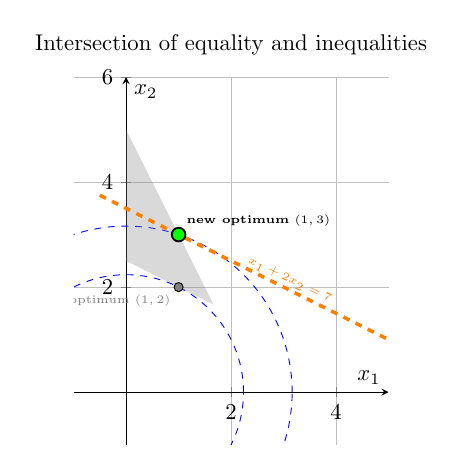
\begin{tikzpicture}[scale=0.82]
\begin{axis}[
  axis lines = middle,
  xlabel = $x_1$,
  ylabel = $x_2$,
  xmin = -1, xmax = 5,
  ymin = -1, ymax = 6,
  axis equal image,
  grid = major,
  title = {Intersection of equality and inequalities}
]
  \draw[blue, dashed] (axis cs:0,0) circle [radius=2.236];
  \draw[blue, dashed] (axis cs:0,0) circle [radius=3.162];

  \fill[gray, opacity=0.3] (axis cs:0, 2.5) -- (axis cs:0, 5) -- (axis cs:1.666, 1.666) -- cycle;

  \addplot[domain=-0.5:5, color=orange, ultra thick, dashed] {3.5 - 0.5*x};
  \node[orange, font=\tiny, rotate=-26, anchor=south] at (axis cs: 3, 1.9) { $x_1 + 2x_2 = 7$};

  \fill[gray, draw=black] (axis cs:1, 2) circle (2pt);
  \node[gray, font=\tiny, anchor=north east] at (axis cs:1, 2) {old optimum $(1,2)$};

  \fill[green, draw=black, thick] (axis cs:1, 3) circle (3pt);
  \node[anchor=south west] at (axis cs:1, 3) {\tiny \textbf{new optimum} $(1,3)$};
\end{axis}
\end{tikzpicture}
\end{center}

\begin{alertbox}{The cost of constraints}
Adding constraints restricts freedom and typically \textbf{increases} the minimum achievable cost.
\end{alertbox}
\end{frame}

% =========================================================
% Classification II: Mathematical structure
% =========================================================
\subsection{Classification II: Mathematical structure}

\begin{frame}{Problem classes (structure)}
\begin{itemize}
  \item \textbf{LP:} linear objective + linear constraints (fast, robust).
  \item \textbf{QP:} quadratic objective + linear constraints (standard linear MPC).
  \item \textbf{Nonconvex QP:} indefinite quadratic (harder; local minima).
  \item \textbf{MILP/MIP:} integer variables + linear structure (combinatorial; expensive).
\end{itemize}
\end{frame}

% ---------------- LP ----------------
\begin{frame}{Linear programmes (LPs)}
Standard form:
\begin{equation*}
\begin{aligned}
\min_x\quad & c^\top x\\
\text{s.t.}\quad &Gx\le h\\
&Ax=b
\end{aligned}
\end{equation*}

\begin{itemize}
  \item Feasible set is a polyhedron.
  \item If an optimum exists, it occurs at an extreme point (vertex).
\end{itemize}
\end{frame}

\begin{frame}{LP geometry: shifting cost hyperplanes}
\begin{center}
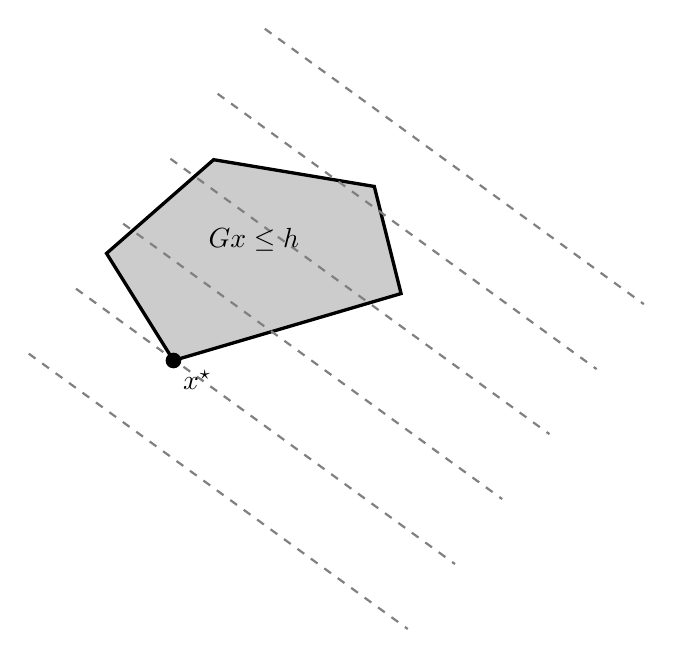
\begin{tikzpicture}[scale=1.7]
  \coordinate (A) at (0.5, 0);
  \coordinate (B) at (0, 0.8);
  \coordinate (C) at (0.8, 1.5);
  \coordinate (D) at (2, 1.3);
  \coordinate (E) at (2.2, 0.5);

  \fill[gray!40] (A) -- (B) -- (C) -- (D) -- (E) -- cycle;
  \draw[line width=1.2pt] (A) -- (B) -- (C) -- (D) -- (E) -- cycle;

  \foreach \y in {-0.3, 0.3, 0.9, 1.5, 2.1, 2.7} {
    \draw[dashed, gray, rotate = -36, thick] (-0.5, \y) -- (3, \y);
  }

  \node at (1.1, 0.9) { $Gx \le h$};
  \node[circle, fill=black, inner sep=2pt] at (A) {};
  \node[below right] at (A) {$x^\star$};
\end{tikzpicture}
\end{center}
\end{frame}

\begin{frame}{LP example: minimum-effort steady state}
\begin{examplebox}{Goal}
For $x_{k+1}=Ax_k+Bu_k$, find an equilibrium $(x_{\mathrm{ss}},u_{\mathrm{ss}})$ satisfying constraints,
with minimum control effort (fuel).
\end{examplebox}

\textbf{Effort as 1-norm:}
\begin{equation*}
\|u\|_1=\sum_{i=1}^m |u_i|
\end{equation*}

\textbf{Epigraph trick:} introduce $t\in\R^m$ with $-t\le u\le t$ and minimise $\mathbf{1}^\top t$.
\end{frame}

\begin{frame}{LP example: full formulation (with norm linearisation)}
\begin{equation*}
\begin{aligned}
\min_{u,\,x_{\mathrm{ss}},\,t}\quad & \mathbf{1}^\top t\\
\text{s.t.}\quad
&(I-A)x_{\mathrm{ss}}-Bu=0 \qquad \text{(equilibrium)}\\
&Gx_{\mathrm{ss}}\le h \qquad \text{(safety)}\\
&u_{\min}\le u\le u_{\max} \qquad \text{(actuator)}\\
&-t\le u\le t \qquad \text{(linearise }|u|\text{)}
\end{aligned}
\end{equation*}

\begin{notebox}{Why this matters in MPC}
Many ``nonlinear-looking'' penalties can be turned into LP/QP-friendly forms by adding auxiliary variables.
\end{notebox}
\end{frame}

\begin{frame}{Stigler's Diet Problem (2D simplified)}
\begin{examplebox}{Decision variables}
$x_1$ = Corn [kg], $x_2$ = Wheat Bread [kg].
\end{examplebox}

\textbf{Objective:} minimise cost $J=c_1x_1+c_2x_2$.

\textbf{Constraints:}
\begin{itemize}
  \item Energy (kcal): $K_{\min}\le k_1x_1+k_2x_2\le K_{\max}$
  \item Vitamin A ($\mu$g): $V_{\min}\le v_1x_1+v_2x_2\le V_{\max}$
  \item Nonnegativity: $x_1,x_2\ge 0$
\end{itemize}
\end{frame}

\begin{frame}{Stigler data (this simplified instance)}
\textbf{Data:}
\begin{itemize}
  \item Costs: $c_1=2.0$, $c_2=0.5$ [\$/kg]
  \item Energy: $k_1=750$, $k_2=650$ (target: $2000$--$3000$ kcal)
  \item Vitamin A: $v_1=250$, $v_2=0$ (target: $500$--$800$ $\mu$g)
\end{itemize}

\begin{equation*}
\begin{aligned}
\min_{x_1,x_2}\quad & 2x_1+0.5x_2\\
\text{s.t.}\quad &2000\le 750x_1+650x_2\le 3000\\
&500\le 250x_1\le 800\\
&x_1\ge 0,\ x_2\ge 0
\end{aligned}
\end{equation*}
\end{frame}

\begin{frame}[fragile]{Stigler in MATLAB/YALMIP}
\scriptsize
\begin{lstlisting}[caption=Solving Stigler's Problem with YALMIP]
clear; clc;

x1 = sdpvar(1); % Corn (kg)
x2 = sdpvar(1); % Bread (kg)

Objective = 2*x1 + 0.5*x2;

Constraints = [];
Constraints = [Constraints, 2000 <= 750*x1 + 650*x2 <= 3000];
Constraints = [Constraints, 500  <= 250*x1           <= 800 ];
Constraints = [Constraints, x1 >= 0, x2 >= 0];

options = sdpsettings('verbose', 0, 'solver', 'linprog');
sol = optimize(Constraints, Objective, options);

if sol.problem == 0
  fprintf('x1 (Corn) : %.4f kg\n', value(x1));
  fprintf('x2 (Bread): %.4f kg\n', value(x2));
  fprintf('Min Cost  : $%.4f\n', value(Objective));
else
  disp('Problem could not be solved.');
end
\end{lstlisting}
\end{frame}

\begin{frame}{Stigler: feasible set and optimum (your provided figure)}
\begin{center}
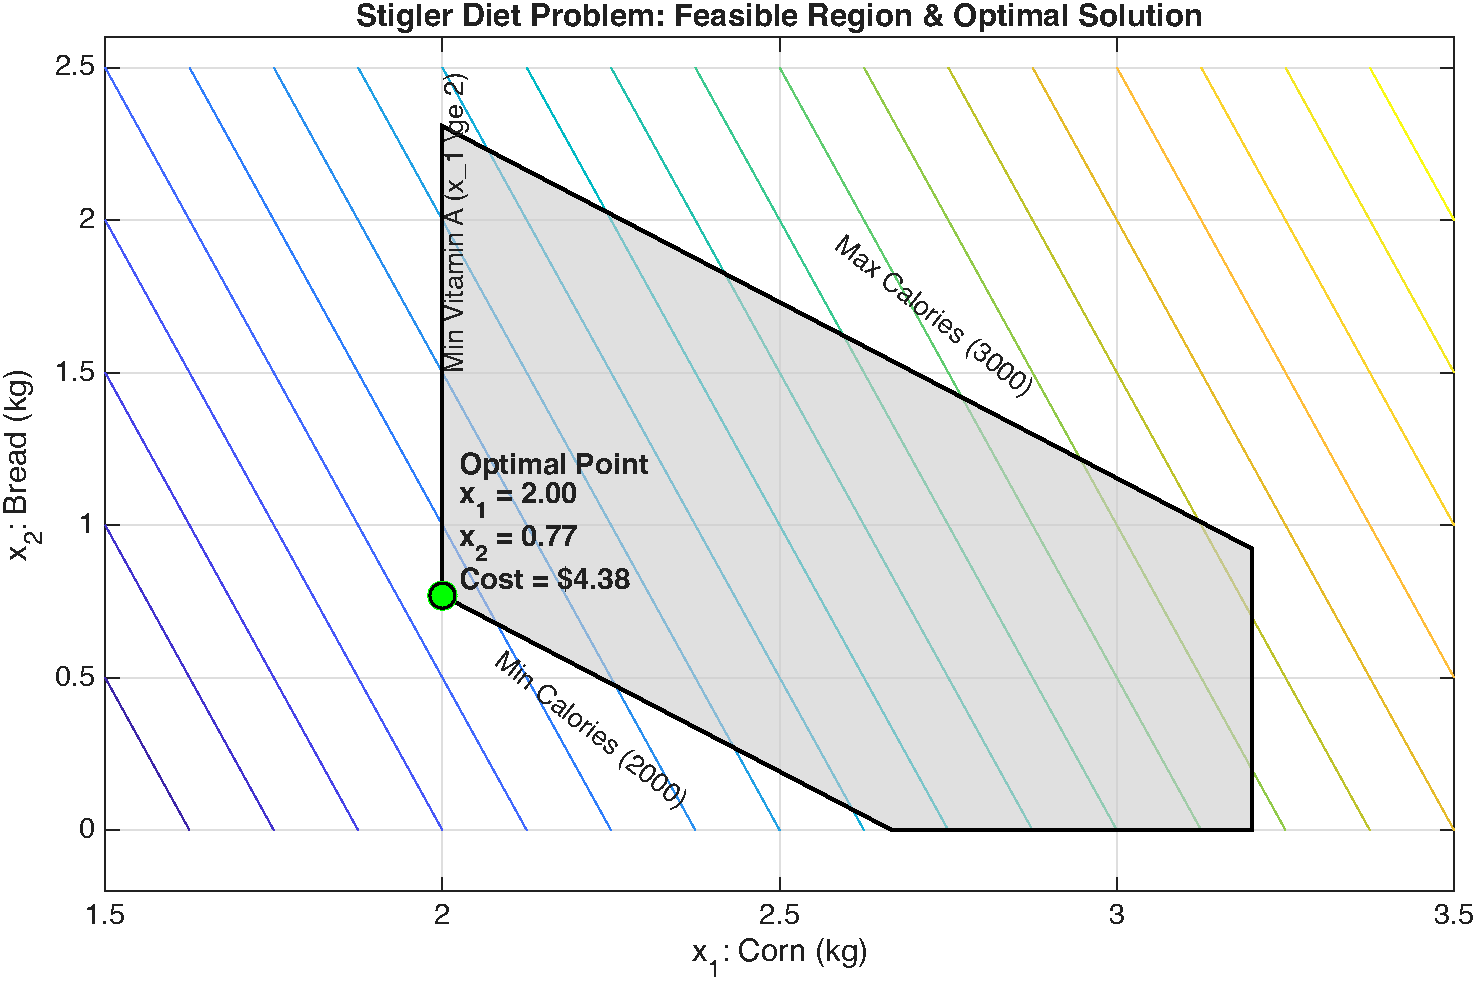
\includegraphics[width=0.75\linewidth,height=0.8\textheight,keepaspectratio]{Stigler2d}
\end{center}
\end{frame}

% ---------------- QP ----------------
\begin{frame}{Convex quadratic programmes (QPs)}
Standard QP:
\begin{equation*}
\begin{aligned}
\min_x\quad &\frac{1}{2}x^\top P x + q^\top x\\
\text{s.t.}\quad &Gx\le h\\
&Ax=b
\end{aligned}
\end{equation*}
Convex iff $P\succeq 0$ (positive semidefinite).
\end{frame}

\begin{frame}{How to test $P\succeq 0$ (positive semidefinite)}
\begin{notebox}{Equivalent tests (for symmetric $P$)}
\begin{enumerate}
  \item All eigenvalues are nonnegative: $\lambda_i(P)\ge 0$.
  \item Quadratic form is nonnegative: $z^\top P z\ge 0,\ \forall z$.
  \item All leading principal minors have nonnegative determinant.
\end{enumerate}
\end{notebox}
\end{frame}

\begin{frame}{The Hessian}
\begin{defnbox}{Hessian}
For $f:\R^n\to\R$, the Hessian $H(x)=\nabla^2 f(x)$ collects second partial derivatives:
\begin{equation*}
H_{ij}=\frac{\partial^2 f}{\partial x_i\,\partial x_j}.
\end{equation*}
For smooth $f$, $H$ is symmetric.
\end{defnbox}
\end{frame}

\begin{frame}{Example: computing a Hessian}
For
\begin{equation*}
f(x)=3x_1^2 + 2x_1x_2 + 5x_2^2,
\end{equation*}
\textbf{Gradient:}
\begin{equation*}
\frac{\partial f}{\partial x_1}=6x_1+2x_2,\qquad
\frac{\partial f}{\partial x_2}=2x_1+10x_2.
\end{equation*}
\textbf{Hessian:}
\begin{equation*}
H=\begin{bmatrix}
6 & 2\\
2 & 10
\end{bmatrix}.
\end{equation*}
\end{frame}

\begin{frame}{QP geometry: ellipses + polytope}
\begin{center}
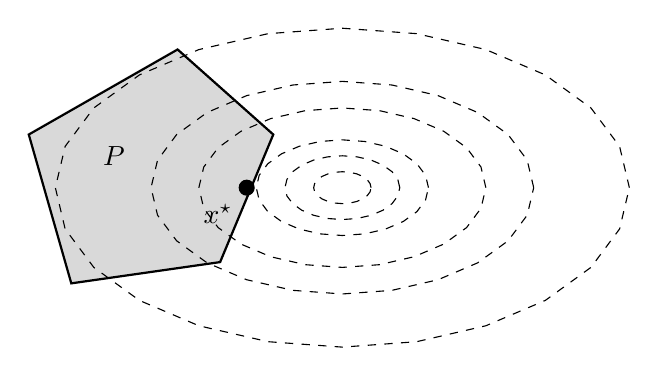
\begin{tikzpicture}[scale=1.35]
  \fill[gray!30]
  (0,0) -- (1.4,0.2) -- (1.9,1.4) -- (1.0,2.2) -- (-0.4,1.4) -- cycle;
  \draw[black, thick]
  (0,0) -- (1.4,0.2) -- (1.9,1.4) -- (1.0,2.2) -- (-0.4,1.4) -- cycle;

  \foreach \s in {0.6,1.2,1.8,3,4,6} {
    \draw[dashed, domain=0:360]
      plot ({2.55 + 0.45*\s*cos(\x)}, {0.9 + 0.25*\s*sin(\x)});
  }

  \filldraw[black] (1.65,0.9) circle (2pt);
  \node at (1.38,0.65) {$x^\star$};
  \node at (0.4,1.2) {$P$};
\end{tikzpicture}
\end{center}

\begin{notebox}{Interpretation}
For strictly convex $P\succ 0$, the global minimiser is unique (if feasible set nonempty).
\end{notebox}
\end{frame}

\begin{frame}{QP example: distance to a restricted zone (setup)}
\begin{examplebox}{Scenario}
Robot at $p=(3,2)$. Restricted zone $\mathcal{X}$ is a unit box centered at origin:
$-1\le x_1\le 1$, $-1\le x_2\le 1$.
\end{examplebox}

\textbf{Goal:} find closest point in the box:
\begin{equation*}
\min_{x\in\mathcal{X}} (x_1-3)^2 + (x_2-2)^2.
\end{equation*}
\end{frame}

\begin{frame}{QP example: geometry (closest point)}
\begin{center}
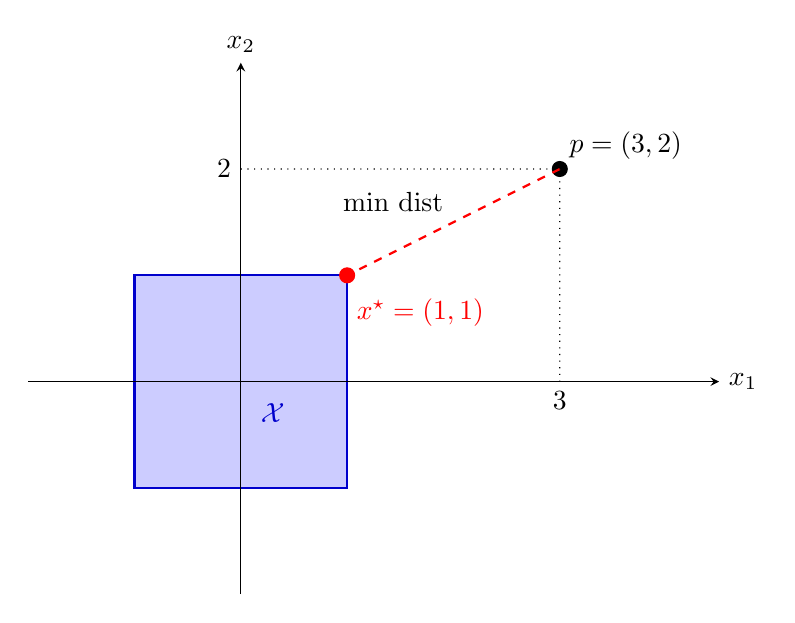
\begin{tikzpicture}[scale=1.35, >=stealth]
  \filldraw[fill=blue!20, draw=blue!80!black, thick] (-1, -1) rectangle (1, 1);
  \node[blue!80!black] at (0.3, -0.3) {$\mathcal{X}$};

  \coordinate (P) at (3, 2);
  \filldraw[black] (P) circle (2pt) node[above right] {$p=(3,2)$};

  \coordinate (Sol) at (1, 1);
  \filldraw[red] (Sol) circle (2pt) node[below right, yshift=-5pt] {$x^\star=(1,1)$};

  \draw[red, dashed, thick] (P) -- (Sol) node[midway, above left, text=black] {min dist};

  \draw[dotted] (3, 0) node[below] {$3$} -- (P);
  \draw[dotted] (0, 2) node[left] {$2$} -- (P);

  \draw[->] (-2, 0) -- (4.5, 0) node[right] {$x_1$};
  \draw[->] (0, -2) -- (0, 3) node[above] {$x_2$};
\end{tikzpicture}
\end{center}
\end{frame}

\begin{frame}{QP example: derive $P,q,G,h$ (standard form)}
Expand objective:
\begin{align*}
J(x) &= (x_1-3)^2+(x_2-2)^2\\
&= x_1^2+x_2^2 - 6x_1 - 4x_2 + 13.
\end{align*}
Drop constant 13 and match $\frac{1}{2}x^\top P x + q^\top x$:
\begin{equation*}
P=\begin{bmatrix}2&0\\0&2\end{bmatrix},\qquad q=\begin{bmatrix}-6\\-4\end{bmatrix}.
\end{equation*}

Box constraints $-1\le x_i\le 1$ become $Gx\le h$:
\begin{equation*}
G=\begin{bmatrix}
1&0\\-1&0\\0&1\\0&-1
\end{bmatrix},\qquad
h=\begin{bmatrix}1\\1\\1\\1\end{bmatrix}.
\end{equation*}
\end{frame}

\begin{frame}[fragile]{QP example: MATLAB/YALMIP (quadprog backend)}
\begin{lstlisting}[caption={Solving the robot distance QP using YALMIP + quadprog.}]
clear; clc;
ops = sdpsettings('solver', 'quadprog', 'verbose', 0);

p = [3; 2];          % Robot position
x = sdpvar(2, 1);    % Decision variable

Objective  = (x(1) - p(1))^2 + (x(2) - p(2))^2;
Constraints = [-1 <= x <= 1];

optimize(Constraints , Objective, ops);

x_opt = value(x);
fprintf('Optimal Sol : x1=%.2f, x2=%.2f\n', x_opt(1), x_opt(2));
\end{lstlisting}
\end{frame}

\begin{frame}[fragile]{QP example: direct quadprog matrices (opening the black box)}
MATLAB \texttt{quadprog} expects:
\begin{equation*}
\min_x\ \frac{1}{2}x^\top Hx + f^\top x\quad \text{s.t.}\quad Ax\le b.
\end{equation*}

\begin{lstlisting}[caption={Direct solution using MATLAB's quadprog.}]
clear; clc;

% Objective: 1/2*x'*P*x + q'*x
H = [2, 0;
     0, 2];          % P
f = [-6; -4];        % q

% Constraints: G*x <= h
A = [ 1,  0;
     -1,  0;
      0,  1;
      0, -1];        % G
b = [1; 1; 1; 1];    % h

options = optimoptions('quadprog', 'Display', 'off');
x_opt = quadprog(H, f, A, b, [], [], [], [], [], options);

fprintf('Optimal Sol : x1=%.2f, x2=%.2f\n', x_opt(1), x_opt(2));
\end{lstlisting}
\end{frame}

\begin{frame}{The QP is the workhorse of linear MPC}
\begin{defnbox}{Why QPs dominate MPC}
Linear MPC with a quadratic cost function and linear constraints produces a \textbf{convex QP} at every time step:
\[
\min_{U} \; \frac{1}{2} U^\top H\, U + f^\top U \quad \text{s.t.} \quad G\, U \le h
\]
where $U = [u_0^\top, u_1^\top, \dots, u_{N-1}^\top]^\top$ is the stacked input sequence.
\end{defnbox}

\vspace{0.3em}
\textbf{Key properties:}
\begin{itemize}
  \item $H \succ 0$ (positive definite) $\Rightarrow$ unique global minimum exists.
  \item QP solvers (\texttt{quadprog}, OSQP, qpOASES) can solve problems with hundreds of variables in milliseconds.
  \item The QP structure is \emph{the same} at every time step --- only the parameters change (current state $x_k$).
  \item This enables \textbf{warm-starting}: using the previous solution as an initial guess.
\end{itemize}
\end{frame}

% ---------------- Nonconvex QP ----------------
\begin{frame}{Nonconvex quadratic programmes}
If $P\not\succeq 0$ (indefinite), the objective is nonconvex:
\begin{equation*}
\min_x\ \frac{1}{2}x^\top Px + q^\top x \quad \text{s.t.}\quad Gx\le h,\ Ax=b.
\end{equation*}

\begin{itemize}
  \item May have multiple local minima and saddle points.
  \item Global optimality is hard to guarantee efficiently.
  \item Standard linear MPC avoids this by using convex QPs.
\end{itemize}
\end{frame}

\begin{frame}{Nonconvex QP: saddle-shaped contours (sketch)}
\begin{center}
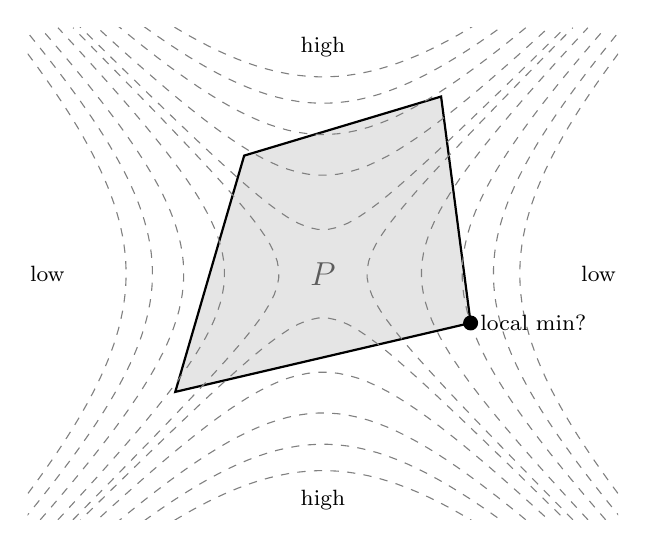
\begin{tikzpicture}[scale=1.25]
  \clip (-3,-2.5) rectangle (3,2.5);

  \coordinate (P1) at (-1.5, -1.2);
  \coordinate (P2) at (1.5, -0.5);
  \coordinate (P3) at (1.2, 1.8);
  \coordinate (P4) at (-0.8, 1.2);

  \fill[gray!40, opacity=0.5] (P1) -- (P2) -- (P3) -- (P4) -- cycle;
  \draw[thick, black] (P1) -- (P2) -- (P3) -- (P4) -- cycle;
  \node at (0,0) [font=\large, opacity=0.6] {$P$};

  \foreach \k in {0.2, 1, 2, 3, 4} {
    \draw[dashed, gray] plot[domain=-3:3, samples=60] (\x, {sqrt(\x*\x + \k)});
    \draw[dashed, gray] plot[domain=-3:3, samples=60] (\x, {-sqrt(\x*\x + \k)});
  }
  \foreach \k in {0.2, 1, 2, 3, 4} {
    \draw[dashed, gray] plot[domain=-2.5:2.5, samples=60] ({sqrt(\x*\x + \k)}, \x);
    \draw[dashed, gray] plot[domain=-2.5:2.5, samples=60] ({-sqrt(\x*\x + \k)}, \x);
  }

  \filldraw (P2) circle (2pt);
  \node[right, font=\footnotesize] at (P2) {local min?};

  \node[font=\footnotesize, fill=white, inner sep=1pt] at (0, 2.3) {high};
  \node[font=\footnotesize, fill=white, inner sep=1pt] at (0, -2.3) {high};
  \node[font=\footnotesize, fill=white, inner sep=1pt] at (-2.8, 0) {low};
  \node[font=\footnotesize, fill=white, inner sep=1pt] at (2.8, 0) {low};
\end{tikzpicture}
\end{center}
\end{frame}

% ---------------- MILP ----------------
\begin{frame}{Mixed-integer linear programmes (MILPs)}
MILP: linear objective + linear constraints, but some variables are integers/binary:
\begin{equation*}
\begin{aligned}
\min_x\quad & c^\top x\\
\text{s.t.}\quad &Gx\le h,\ Ax=b\\
&x\in\{0,1\}^p\times \R^{n-p}\ \ \text{or}\ \ x\in\Z^p\times\R^{n-p}.
\end{aligned}
\end{equation*}

\begin{alertbox}{Why hard?}
Feasible set becomes \textbf{discrete points} in a polyhedron $\Rightarrow$ combinatorial explosion.
\end{alertbox}
\end{frame}

\begin{frame}{MILP sketch: integer lattice inside a polytope}
\begin{center}
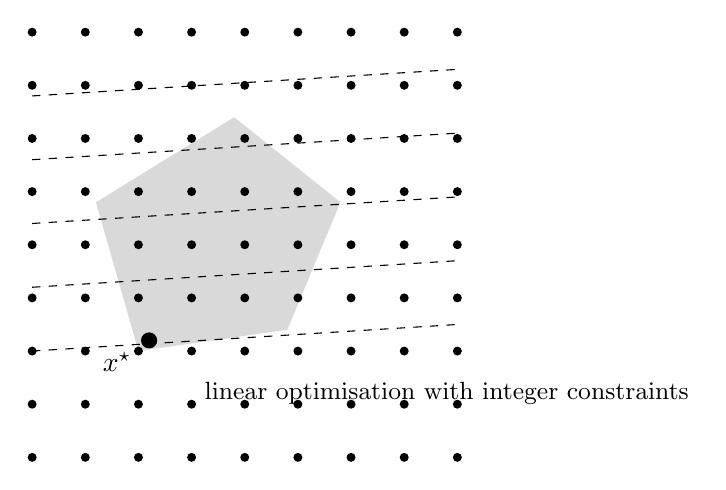
\begin{tikzpicture}[scale=1.35]
  \fill[gray!30] (0,0) -- (1.4,0.2) -- (1.9,1.4) -- (0.9,2.2) -- (-0.4,1.4) -- cycle;

  \foreach \xx in {-1,-0.5,...,3} {
    \foreach \yy in {-1,-0.5,...,3} {
      \fill (\xx,\yy) circle (1.2pt);
    }
  }

  \foreach \yy in {0.0,0.6,1.2,1.8,2.4} {
    \draw[dashed] (-1,\yy) -- (3,\yy+0.25);
  }

  \filldraw[black] (0.1,0.1) circle (2pt);
  \node at (-0.2,-0.1) {$x^\star$};
  \node at (2.9,-0.4) {\small linear optimisation with integer constraints};
\end{tikzpicture}
\end{center}
\end{frame}

\begin{frame}{MILP example: industrial energy management (model structure)}
\begin{examplebox}{Idea}
Grid + generator + battery. Minimise operating cost while meeting demand.
\end{examplebox}

At each time step $k=1,\dots,N$, typical variables include:
\begin{itemize}
  \item Continuous: $p_g(k), p_{\mathrm{grid}}(k), p_{\mathrm{ch}}(k), p_{\mathrm{dis}}(k), E(k)$
  \item Binary logic: $u(k)$ on/off, $s(k)$ start-up, $z(k)$ charge-mode
\end{itemize}

\begin{alertbox}{MILP drivers}
Binary variables make the problem mixed-integer \(\Rightarrow\) need solvers like Gurobi/CPLEX.
\end{alertbox}
\end{frame}

% =========================================================
% Software tools
% =========================================================
\section{Software tools for optimisation}

\begin{frame}{Two-layer software stack}
\begin{enumerate}
  \item \textbf{Parsers / modelling languages:} translate symbolic constraints/objectives to matrices.
  \item \textbf{Solvers:} numerical engines (active-set, interior point, ADMM, etc.).
\end{enumerate}

\begin{notebox}{Why you should care}
Understanding the mapping from maths $\rightarrow$ matrices $\rightarrow$ solver inputs helps you debug and design MPC effectively.
\end{notebox}
\end{frame}

\begin{frame}{Modelling languages (parsers)}
\scriptsize
\begin{table}
\centering
\renewcommand{\arraystretch}{1.15}
\begin{tabularx}{\linewidth}{@{}l l l X@{}}
\toprule
\textbf{Name} & \textbf{Platform} & \textbf{License} & \textbf{Primary purpose / notes}\\
\midrule
YALMIP & MATLAB & Free & Flexible modelling for LP/QP/SDP/MIP; great for prototyping.\\
CVX & MATLAB & Free & Disciplined convex programming (DCP); strong convexity guarantees.\\
CVXPY & Python & Free (Apache) & Python equivalent of CVX; clean OO interface for convex problems.\\
CasADi & Python/C++/MATLAB & Free (LGPL) & Nonlinear MPC; algorithmic differentiation; C-code generation.\\
Pyomo & Python & Free (BSD) & General operations research modelling; wide solver support.\\
JuMP & Julia & Free (MIT) & Very fast modelling; popular in optimisation/control community.\\
\bottomrule
\end{tabularx}
\end{table}
\end{frame}

\begin{frame}{Numerical solvers (what they are good for)}
\scriptsize
\begin{table}
\centering
\renewcommand{\arraystretch}{1.12}
\begin{tabularx}{\linewidth}{@{}l l l l X@{}}
\toprule
\textbf{Solver} & \textbf{Type} & \textbf{Method} & \textbf{License} & \textbf{Best for}\\
\midrule
quadprog & QP & Interior-point & Proprietary & Standard MATLAB QP (course default; Opt Toolbox).\\
OSQP & QP & ADMM & Free (Apache) & Embedded MPC; robust, fast to medium accuracy.\\
qpOASES & QP & Active-set & Free (LGPL) & MPC warm-starting; small/medium dense QPs.\\
Gurobi & LP/QP/MIP & Barrier/Simplex & Commercial & Very fast large-scale convex + MIP (acad. licenses).\\
MOSEK & SOCP/SDP & Interior-point & Commercial & Conic/robust MPC; LMIs/SDP.\\
SeDuMi & SOCP/SDP & Interior-point & Free (GPL) & Classic MATLAB LMI/SDP solver.\\
IPOPT & NLP & Interior-point & Free (EPL) & Large-scale nonlinear optimisation (NMPC).\\
SNOPT & NLP & SQP & Commercial & Difficult nonconvex NLPs (e.g. trajectories).\\
ECOS & SOCP/LP & Interior-point & Free (GPL) & Lightweight conic solver, embedded friendly.\\
\bottomrule
\end{tabularx}
\end{table}
\end{frame}

\begin{frame}{YALMIP: the five-step workflow}
\begin{enumerate}
  \item \textbf{Define variables:} \texttt{x = sdpvar(n, 1)}
  \item \textbf{Define objective:} \texttt{J = x'*Q*x + c'*x}
  \item \textbf{Define constraints:} \texttt{C = [A*x <= b, x >= 0]}
  \item \textbf{Solve:} \texttt{optimize(C, J, sdpsettings('solver','quadprog'))}
  \item \textbf{Extract solution:} \texttt{x\_opt = value(x)}
\end{enumerate}

\vspace{0.5em}
\begin{notebox}{Why use YALMIP instead of calling solvers directly?}
\begin{itemize}
  \item You write maths, YALMIP writes matrices --- fewer bugs.
  \item Same code works with different solvers (just change the solver name).
  \item Automatic detection of problem type (LP, QP, SDP, \ldots).
  \item The \texttt{optimizer} object pre-compiles the problem for fast repeated solves (essential for MPC).
\end{itemize}
\end{notebox}
\end{frame}

% =========================================================
% From theory to code: Economic MPC example
% =========================================================
\section{From theory to code: an Economic MPC example}

\begin{frame}{Economic MPC for smart grids (battery arbitrage)}
\begin{examplebox}{Scenario}
Home with load $P_{\mathrm{load}}$, solar $P_{\mathrm{solar}}$, battery energy $E_{\mathrm{bat}}$, grid exchange $P_{\mathrm{grid}}$.
Prices vary throughout the day.
\end{examplebox}

\textbf{Goal:} choose charge/discharge schedule to minimise daily electricity cost over $N=24$ hours.
\end{frame}

\begin{frame}{Model (variables, objective, constraints)}
Let $\Delta t=1$ hour and $k=0,\dots,N-1$.

\textbf{Variables:}
\begin{itemize}
  \item $P_{\mathrm{grid}}(k)$: grid power (+buy, -sell)
  \item $P_{\mathrm{bat}}(k)$: battery power (+charge, -discharge)
  \item $E_{\mathrm{bat}}(k)$: stored energy
\end{itemize}

\textbf{Objective:}
\begin{equation*}
\min \sum_{k=0}^{N-1} \mathrm{Price}(k)\,P_{\mathrm{grid}}(k)\,\Delta t
\end{equation*}

\textbf{Constraints:}
\begin{align*}
P_{\mathrm{grid}}(k)+P_{\mathrm{solar}}(k)&=P_{\mathrm{load}}(k)+P_{\mathrm{bat}}(k)\\
E_{\mathrm{bat}}(k+1)&=E_{\mathrm{bat}}(k)+P_{\mathrm{bat}}(k)\Delta t\\
E_{\min}\le E_{\mathrm{bat}}(k)&\le E_{\max},\qquad
P_{\min}\le P_{\mathrm{bat}}(k)\le P_{\max}
\end{align*}
\end{frame}

\begin{frame}[fragile]{MATLAB/YALMIP implementation (battery arbitrage LP) 1/2}
\scriptsize
\begin{lstlisting}
% --- 1. System Parameters ---
N = 24;                 % Horizon (24 hours)
E_cap = 13.5;           % Battery Capacity (kWh)
P_max = 5;              % Max Charge/Discharge rate (kW)
dt = 1;                 % Time step (1 hour)

% --- 2. Forecast Data (Profiles) ---
Price = 0.10 * ones(N,1);
Price(18:21) = 0.30;    % Peak 17:00--21:00 (1-indexed hours)

t = (0:N-1)';
Solar = max(0, 4 * sin(pi * (t - 6) / 12));  % simple solar profile
Load  = 1 + 2 * exp(-(t-19).^2/10) + 1 * exp(-(t-8).^2/5);

% --- 3. Optimisation Variables ---
P_grid = sdpvar(N, 1);
P_bat  = sdpvar(N, 1);
E_bat  = sdpvar(N+1, 1);
\end{lstlisting}
\end{frame}


\begin{frame}[fragile]{MATLAB/YALMIP implementation (battery arbitrage LP) 2/2}
	\scriptsize
	\begin{lstlisting}
			:
			:
			:
		
		% --- 4. Constraints ---
		C = [];
		C = [C, E_bat(1) == 0];  % initial SoC (in MPC use measurement)
		
		for k = 1:N
		C = [C, E_bat(k+1) == E_bat(k) + P_bat(k)*dt];
		C = [C, P_grid(k) + Solar(k) == Load(k) + P_bat(k)];
		C = [C, 0 <= E_bat(k+1) <= E_cap];
		C = [C, -P_max <= P_bat(k) <= P_max];
		end
		
		% --- 5. Objective ---
		Objective = Price' * P_grid;
		
		% --- 6. Solve ---
		ops = sdpsettings('solver','quadprog','verbose',0);
		sol = optimize(C, Objective, ops);
	\end{lstlisting}
\end{frame}


\begin{frame}{Result visualisation (your provided figure)}
\begin{center}
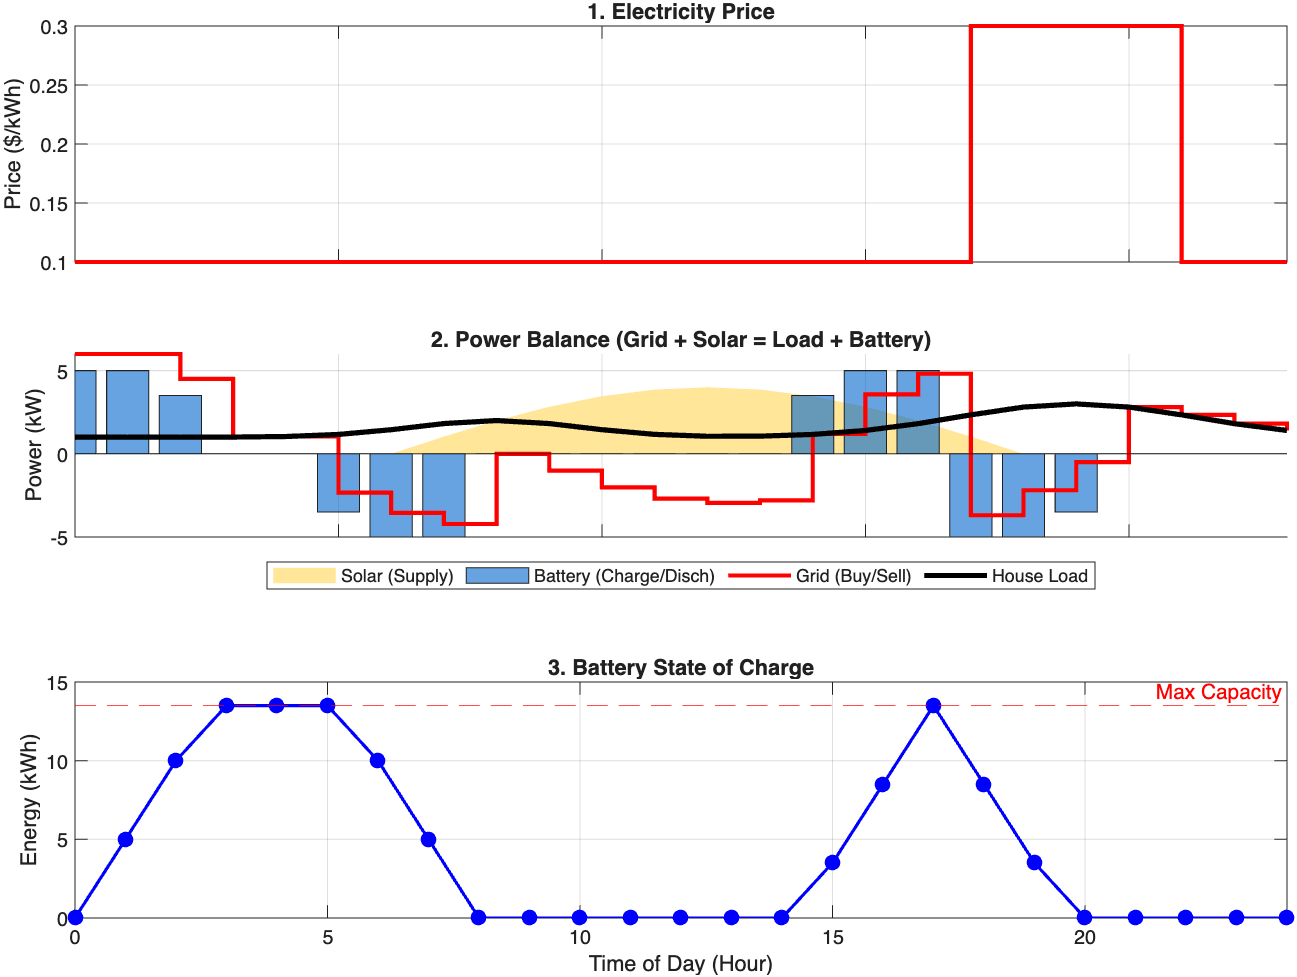
\includegraphics[width=0.85\linewidth,height=0.75\textheight,keepaspectratio]{energy_management}
\end{center}
\end{frame}

\begin{frame}{Interpreting the result}
\begin{enumerate}
  \item \textbf{Pre-charging:} at low prices (night), the optimiser buys electricity to charge the battery.
  \item \textbf{Peak shaving / arbitrage:} during high price window, it discharges (and may sell) to avoid expensive grid usage.
  \item \textbf{Constraint realism:} $E_{\mathrm{bat}}$ and $P_{\mathrm{bat}}$ limits shape what is achievable.
\end{enumerate}

\begin{notebox}{MPC connection}
In closed-loop MPC, the forecast profiles are updated each step and the initial $E_{\mathrm{bat}}(1)$ comes from sensors.
\end{notebox}
\end{frame}

% =========================================================
% Key takeaways
% =========================================================
\section{Key takeaways}

\begin{frame}{Chapter summary: the optimisation landscape}
\begin{center}
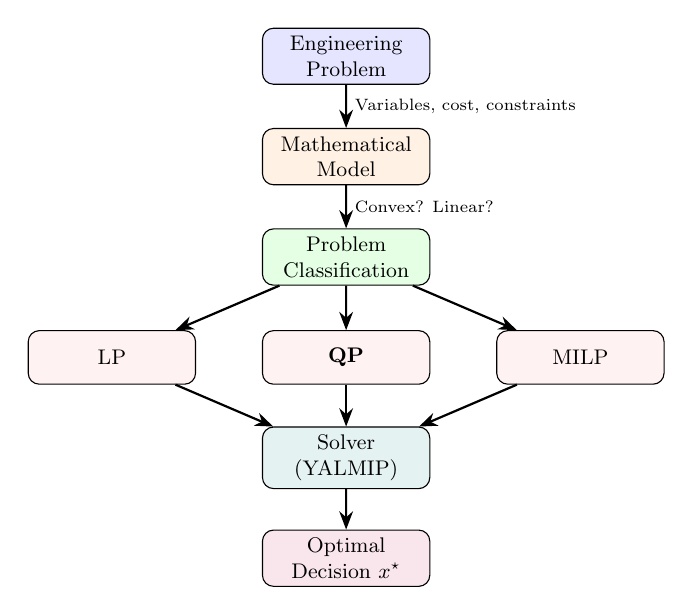
\begin{tikzpicture}[scale=0.85, transform shape,
  every node/.style={font=\small},
  box/.style={draw, rounded corners, minimum width=2.5cm, minimum height=0.8cm, align=center},
  arrow/.style={-Stealth, thick}
]
  \node[box, fill=blue!10] (eng) at (0,3) {Engineering\\Problem};
  \node[box, fill=orange!10] (model) at (0,1.5) {Mathematical\\Model};
  \node[box, fill=green!10] (class) at (0,0) {Problem\\Classification};

  \node[box, fill=red!5] (lp) at (-3.5,-1.5) {LP};
  \node[box, fill=red!5] (qp) at (0,-1.5) {\textbf{QP}};
  \node[box, fill=red!5] (milp) at (3.5,-1.5) {MILP};

  \node[box, fill=teal!10] (solver) at (0,-3) {Solver\\(YALMIP)};
  \node[box, fill=purple!10] (sol) at (0,-4.5) {Optimal\\Decision $x^\star$};

  \draw[arrow] (eng) -- (model) node[midway,right] {\scriptsize Variables, cost, constraints};
  \draw[arrow] (model) -- (class) node[midway,right] {\scriptsize Convex? Linear?};
  \draw[arrow] (class) -- (lp);
  \draw[arrow] (class) -- (qp);
  \draw[arrow] (class) -- (milp);
  \draw[arrow] (lp) -- (solver);
  \draw[arrow] (qp) -- (solver);
  \draw[arrow] (milp) -- (solver);
  \draw[arrow] (solver) -- (sol);
\end{tikzpicture}
\end{center}
\end{frame}

\begin{frame}{Key takeaways (1/2)}
\begin{itemize}
  \item \textbf{Optimisation is translation:} from qualitative goals to quantitative maths.
  \item \textbf{Scalar score:} algorithms minimise a single number; $J(x)$ ranks plans.
  \item \textbf{Constraints define reality:} feasibility is the intersection of all constraints.
  \item \textbf{Infeasible} problems have no solution; modelling matters.
\end{itemize}
\end{frame}

\begin{frame}{Key takeaways (2/2)}
\begin{itemize}
  \item \textbf{Convexity is king:} convex objective + convex feasible set $\Rightarrow$ local min is global min.
  \item \textbf{Standard forms matter:}
  \begin{itemize}
    \item LP: very fast; economic dispatch / simple regulation.
    \item QP: standard linear MPC (energy/error costs) with linear constraints.
    \item MILP: logic/on-off decisions; powerful but computationally expensive.
  \end{itemize}
  \item \textbf{Max $\leftrightarrow$ min:} $\argmax f(x)\equiv \argmin (-f(x))$.
\end{itemize}
\end{frame}

\begin{frame}{Next steps (bridge to MPC formulations)}
\begin{itemize}
  \item In MPC, decision vector becomes a stacked input sequence $U = [u_0^\top,u_1^\top,\dots,u_{N-1}^\top]^\top$.
  \item Dynamics appear as equality constraints across the horizon.
  \item Standard linear MPC leads to a \textbf{convex QP} solved every sampling time.
  \item Warm-starting and solver selection are practical performance levers.
\end{itemize}
\end{frame}

\section{Exercises for self-study}

\begin{frame}{Exercises for self-study (1/2)}
\textbf{Exercise 1: Convex sets and functions.}
\begin{itemize}
  \item Determine whether the following sets are convex:
    \begin{enumerate}
      \item $\{x \in \R^2 \mid x_1^2 + x_2^2 \le 4\}$
      \item $\{x \in \R^2 \mid x_1^2 + x_2^2 \ge 1\}$
      \item $\{x \in \R^2 \mid 2x_1 + 3x_2 \le 6,\; x_1 \ge 0,\; x_2 \ge 0\}$
    \end{enumerate}
  \item Check whether $f(x) = 5x_1^2 - 4x_1 x_2 + 3x_2^2$ is convex by computing the Hessian eigenvalues.
\end{itemize}

\vspace{0.5em}
\textbf{Exercise 2: Gradient and Hessian.}
\begin{itemize}
  \item For $J(x) = 4x_1^2 + 6x_1 x_2 + 8x_2^2 - 10x_1 + 2x_2$:
  \begin{enumerate}
    \item Compute $\nabla J$, set it to zero, and find the stationary point.
    \item Compute $\nabla^2 J$. Is $J$ convex?
  \end{enumerate}
\end{itemize}
\end{frame}

\begin{frame}{Exercises for self-study (2/2)}
\textbf{Exercise 3: LP formulation.}
\begin{itemize}
  \item A factory makes products A and B. Product A needs 2h on Machine~1 and 3h on Machine~2; product B needs 4h on Machine~1 and 1h on Machine~2. Available: 10h (M1), 12h (M2). Profit: \pounds3/unit (A), \pounds5/unit (B). Formulate as LP.
\end{itemize}

\vspace{0.5em}
\textbf{Exercise 4: QP standard form.}
\begin{itemize}
  \item For $\min_{u} 3u_1^2 + 2u_1 u_2 + 4u_2^2 - 8u_1 - 6u_2$ subject to $u_1 + u_2 \le 5$, $0 \le u_1 \le 3$, $0 \le u_2 \le 4$:
  \begin{enumerate}
    \item Write in standard QP form $\frac{1}{2}u^\top P u + q^\top u$.
    \item Show $P \succ 0$ (convex). Express constraints as $Gu \le h$.
    \item Solve using YALMIP or \texttt{quadprog}.
  \end{enumerate}
\end{itemize}

\vspace{0.5em}
\textbf{Exercise 5: Satellite fuel minimisation.}
\begin{itemize}
  \item Dynamics: $x_{k+1} = Ax_k + Bu_k$. Goal: reach steady state with $\min \|u_{ss}\|_1$, $|u_{ss}| \le 10$.
  \item Show the equilibrium condition, apply the epigraph trick, formulate as LP.
\end{itemize}
\end{frame}

\end{document}
